
\documentclass{article} % For LaTeX2e
% \usepackage[submission]{colm2025_conference}
\usepackage[table]{xcolor}
\usepackage[preprint]{colm2025_conference}
\usepackage{multirow}
\usepackage{microtype}
\usepackage{url}
\usepackage{booktabs}
\usepackage{makecell}
% \usepackage{lineno}
\usepackage{graphicx}
\usepackage[font=small]{caption} % 캡션 폰트 크기 호조절
\usepackage{subfig}
\usepackage{amssymb}
\usepackage{pifont}
\usepackage[most]{tcolorbox}
\usepackage{wrapfig}
\usepackage{float}
\usepackage{longtable}
\usepackage{setspace}
\usepackage{listings}
\usepackage{verbatim}
\usepackage{footnote}
\usepackage{CJKutf8}
\usepackage{kotex}
\usepackage{spverbatim}

\usepackage{hyperref}

\usepackage{tikz}
\usetikzlibrary{tikzmark,positioning}

\definecolor{darkblue}{rgb}{0, 0, 0.5}
\definecolor{yellow}{RGB}{255, 230, 100}
\hypersetup{colorlinks=true, citecolor=darkblue, linkcolor=darkblue, urlcolor=darkblue}



\newcommand{\cmark}{\ding{51}}%
\newcommand{\xmark}{\ding{55}}%


\title{Kanana: Compute-efficient Bilingual Language Models}


\author{\textbf{Kanana LLM Team} \thanks{A detailed contributor list can be found in the last section of the main paper.} \\
\texttt{kanana-llm@kakaocorp.com} \\
}


\newcommand{\fix}{\marginpar{FIX}}
\newcommand{\new}{\marginpar{NEW}}

\begin{document}

\ifcolmsubmission
\linenumbers
\fi

\maketitle


\begin{abstract}
We introduce Kanana, a series of bilingual language models that demonstrate exceeding performance in Korean and competitive performance in English. 
The computational cost of Kanana is significantly lower than that of state-of-the-art models of similar size.
The report details the techniques employed during pre-training to achieve compute-efficient yet competitive models, including high quality data filtering, staged pre-training, depth up-scaling, and pruning and distillation.
Furthermore, the report outlines the methodologies utilized during the post-training of the Kanana models, encompassing supervised fine-tuning and preference optimization, aimed at enhancing their capability for seamless interaction with users.
Lastly, the report elaborates on plausible approaches used for language model adaptation to specific scenarios, such as embedding, retrieval augmented generation, and function calling.
The Kanana model series spans from 2.1B to 32.5B parameters with 2.1B models (base, instruct, embedding) publicly released to promote research on Korean language models.
\end{abstract}


\section{Introduction}
\label{sec:introduction}
The business processes of organizations are experiencing ever-increasing complexity due to the large amount of data, high number of users, and high-tech devices involved \cite{martin2021pmopportunitieschallenges, beerepoot2023biggestbpmproblems}. This complexity may cause business processes to deviate from normal control flow due to unforeseen and disruptive anomalies \cite{adams2023proceddsriftdetection}. These control-flow anomalies manifest as unknown, skipped, and wrongly-ordered activities in the traces of event logs monitored from the execution of business processes \cite{ko2023adsystematicreview}. For the sake of clarity, let us consider an illustrative example of such anomalies. Figure \ref{FP_ANOMALIES} shows a so-called event log footprint, which captures the control flow relations of four activities of a hypothetical event log. In particular, this footprint captures the control-flow relations between activities \texttt{a}, \texttt{b}, \texttt{c} and \texttt{d}. These are the causal ($\rightarrow$) relation, concurrent ($\parallel$) relation, and other ($\#$) relations such as exclusivity or non-local dependency \cite{aalst2022pmhandbook}. In addition, on the right are six traces, of which five exhibit skipped, wrongly-ordered and unknown control-flow anomalies. For example, $\langle$\texttt{a b d}$\rangle$ has a skipped activity, which is \texttt{c}. Because of this skipped activity, the control-flow relation \texttt{b}$\,\#\,$\texttt{d} is violated, since \texttt{d} directly follows \texttt{b} in the anomalous trace.
\begin{figure}[!t]
\centering
\includegraphics[width=0.9\columnwidth]{images/FP_ANOMALIES.png}
\caption{An example event log footprint with six traces, of which five exhibit control-flow anomalies.}
\label{FP_ANOMALIES}
\end{figure}

\subsection{Control-flow anomaly detection}
Control-flow anomaly detection techniques aim to characterize the normal control flow from event logs and verify whether these deviations occur in new event logs \cite{ko2023adsystematicreview}. To develop control-flow anomaly detection techniques, \revision{process mining} has seen widespread adoption owing to process discovery and \revision{conformance checking}. On the one hand, process discovery is a set of algorithms that encode control-flow relations as a set of model elements and constraints according to a given modeling formalism \cite{aalst2022pmhandbook}; hereafter, we refer to the Petri net, a widespread modeling formalism. On the other hand, \revision{conformance checking} is an explainable set of algorithms that allows linking any deviations with the reference Petri net and providing the fitness measure, namely a measure of how much the Petri net fits the new event log \cite{aalst2022pmhandbook}. Many control-flow anomaly detection techniques based on \revision{conformance checking} (hereafter, \revision{conformance checking}-based techniques) use the fitness measure to determine whether an event log is anomalous \cite{bezerra2009pmad, bezerra2013adlogspais, myers2018icsadpm, pecchia2020applicationfailuresanalysispm}. 

The scientific literature also includes many \revision{conformance checking}-independent techniques for control-flow anomaly detection that combine specific types of trace encodings with machine/deep learning \cite{ko2023adsystematicreview, tavares2023pmtraceencoding}. Whereas these techniques are very effective, their explainability is challenging due to both the type of trace encoding employed and the machine/deep learning model used \cite{rawal2022trustworthyaiadvances,li2023explainablead}. Hence, in the following, we focus on the shortcomings of \revision{conformance checking}-based techniques to investigate whether it is possible to support the development of competitive control-flow anomaly detection techniques while maintaining the explainable nature of \revision{conformance checking}.
\begin{figure}[!t]
\centering
\includegraphics[width=\columnwidth]{images/HIGH_LEVEL_VIEW.png}
\caption{A high-level view of the proposed framework for combining \revision{process mining}-based feature extraction with dimensionality reduction for control-flow anomaly detection.}
\label{HIGH_LEVEL_VIEW}
\end{figure}

\subsection{Shortcomings of \revision{conformance checking}-based techniques}
Unfortunately, the detection effectiveness of \revision{conformance checking}-based techniques is affected by noisy data and low-quality Petri nets, which may be due to human errors in the modeling process or representational bias of process discovery algorithms \cite{bezerra2013adlogspais, pecchia2020applicationfailuresanalysispm, aalst2016pm}. Specifically, on the one hand, noisy data may introduce infrequent and deceptive control-flow relations that may result in inconsistent fitness measures, whereas, on the other hand, checking event logs against a low-quality Petri net could lead to an unreliable distribution of fitness measures. Nonetheless, such Petri nets can still be used as references to obtain insightful information for \revision{process mining}-based feature extraction, supporting the development of competitive and explainable \revision{conformance checking}-based techniques for control-flow anomaly detection despite the problems above. For example, a few works outline that token-based \revision{conformance checking} can be used for \revision{process mining}-based feature extraction to build tabular data and develop effective \revision{conformance checking}-based techniques for control-flow anomaly detection \cite{singh2022lapmsh, debenedictis2023dtadiiot}. However, to the best of our knowledge, the scientific literature lacks a structured proposal for \revision{process mining}-based feature extraction using the state-of-the-art \revision{conformance checking} variant, namely alignment-based \revision{conformance checking}.

\subsection{Contributions}
We propose a novel \revision{process mining}-based feature extraction approach with alignment-based \revision{conformance checking}. This variant aligns the deviating control flow with a reference Petri net; the resulting alignment can be inspected to extract additional statistics such as the number of times a given activity caused mismatches \cite{aalst2022pmhandbook}. We integrate this approach into a flexible and explainable framework for developing techniques for control-flow anomaly detection. The framework combines \revision{process mining}-based feature extraction and dimensionality reduction to handle high-dimensional feature sets, achieve detection effectiveness, and support explainability. Notably, in addition to our proposed \revision{process mining}-based feature extraction approach, the framework allows employing other approaches, enabling a fair comparison of multiple \revision{conformance checking}-based and \revision{conformance checking}-independent techniques for control-flow anomaly detection. Figure \ref{HIGH_LEVEL_VIEW} shows a high-level view of the framework. Business processes are monitored, and event logs obtained from the database of information systems. Subsequently, \revision{process mining}-based feature extraction is applied to these event logs and tabular data input to dimensionality reduction to identify control-flow anomalies. We apply several \revision{conformance checking}-based and \revision{conformance checking}-independent framework techniques to publicly available datasets, simulated data of a case study from railways, and real-world data of a case study from healthcare. We show that the framework techniques implementing our approach outperform the baseline \revision{conformance checking}-based techniques while maintaining the explainable nature of \revision{conformance checking}.

In summary, the contributions of this paper are as follows.
\begin{itemize}
    \item{
        A novel \revision{process mining}-based feature extraction approach to support the development of competitive and explainable \revision{conformance checking}-based techniques for control-flow anomaly detection.
    }
    \item{
        A flexible and explainable framework for developing techniques for control-flow anomaly detection using \revision{process mining}-based feature extraction and dimensionality reduction.
    }
    \item{
        Application to synthetic and real-world datasets of several \revision{conformance checking}-based and \revision{conformance checking}-independent framework techniques, evaluating their detection effectiveness and explainability.
    }
\end{itemize}

The rest of the paper is organized as follows.
\begin{itemize}
    \item Section \ref{sec:related_work} reviews the existing techniques for control-flow anomaly detection, categorizing them into \revision{conformance checking}-based and \revision{conformance checking}-independent techniques.
    \item Section \ref{sec:abccfe} provides the preliminaries of \revision{process mining} to establish the notation used throughout the paper, and delves into the details of the proposed \revision{process mining}-based feature extraction approach with alignment-based \revision{conformance checking}.
    \item Section \ref{sec:framework} describes the framework for developing \revision{conformance checking}-based and \revision{conformance checking}-independent techniques for control-flow anomaly detection that combine \revision{process mining}-based feature extraction and dimensionality reduction.
    \item Section \ref{sec:evaluation} presents the experiments conducted with multiple framework and baseline techniques using data from publicly available datasets and case studies.
    \item Section \ref{sec:conclusions} draws the conclusions and presents future work.
\end{itemize}

This section describes our pre-training setup, including details about the data collection and curation process (Section \ref{subsec:pretrain_data}), the challenges faced when training at scale in our distributed environment (Sections \ref{subsec:infra}, \ref{subsec:parallelism} and \ref{subsec:operational_challenges}), and finally, the pre-training recipes used for each model (Sections \ref{subsec:pretrain_method} and \ref{subsec:annealing}).

\subsection{Data}
\label{subsec:pretrain_data}

\begin{figure}[tb]
\vskip 0.1in
\begin{center}
\centerline{\includegraphics[width=\columnwidth]{pictures/pretraining_data.pdf}}
\caption{The composition statistics of pre-training data, including Chinese, English, multilingual, and code.}
\label{pre-training_data}
\end{center}
\vskip -0.3in
\end{figure}

\clearpage
\subsection{Technical Infrastructure}
\label{subsec:infra}
% SGirona slides: https://www.bsc.es/sites/default/files/public/u2416/20230220_marenostrum5_sergi_girona_bsc.pdf

Salamandra was trained in MareNostrum 5\footnote{\url{https://www.bsc.es/marenostrum/marenostrum-5}}, a pre-exascale EuroHPC supercomputer hosted and operated by Barcelona Supercomputing Center. The accelerated partition is based on Intel Sapphire Rapids and Nvidia Hopper GPUs (H100s) \cite{h100}, totaling 1,120 nodes with four 64GB H100 GPUs each. On the other hand, the general-purpose compute partition has 6,480 nodes based on Intel Sapphire Rapids. Each node has 112 cores and 256 GB of main memory. However, for data processing tasks, a small subsystem of high-memory nodes with 1,024 GB was used.

The peak performance is around 46 petaflops for the general-purpose partition and 260 petaflops for the accelerated partition. The network topology is fat-tree in both cases. Inter-node communication uses InfiniBand NDR 200, while the GPUs within each node are connected via NVLink. 

Regarding the storage system, MareNostrum 5 has a total net capacity of 248 PetaBytes on SSD and hard disks. However, during the actual training, data was transferred to the internal memory of each node to optimize input/output (IO) operations and improve processing speed. During our preliminary experiments, we noticed that this would significantly reduce the time spent reading chunks of data from disk, which posed a significant bottleneck.

It is worth mentioning that the node configuration of our accelerated cluster is rather atypical, featuring Nvidia H100 GPUs with 64 GB of VRAM, instead of the more standard 80 GB configuration. Additionally, each node is equipped with 4 GPUs, as opposed to the 8 GPUs commonly found in Nvidia's DGX systems\footnote{\url{https://www.nvidia.com/en-gb/data-center/dgx-h100}}. As will be further detailed in the following section, these hardware features will influence the choice of hyper-parameters for parallelism. Specifically, the reduced VRAM memory limits the model chunks' size, while the lower number of GPUs constrains the level of tensor parallelism that can be achieved.  Consequently, careful tuning of such parameters is necessary to optimize performance within these constraints. 


\subsection{Distributed Training}
\label{subsec:parallelism}
One of the main technical challenges when training large language models at scale is the memory bottleneck imposed by the limited VRAM memory of modern processors. The reason is that, during training, not only the model parameters must be stored in the device's memory, but also the optimizer states, gradients, and activations. As a result, model weights have to be distributed across several devices, which makes parallelism and memory management techniques extremely necessary. We will be using intra-layer tensor parallelism along with inter-layer pipeline parallelism for model sharding, as well as activation checkpointing and flash attention to reduce the memory footprint. 

Another major challenge is compute efficiency, because even if it was possible to fit an entire model in a single GPU, the training time on that sole device would be unrealistically large. Fortunately, this can be easily tackled by employing data parallelism, which consists in distributing several data shards across copies of the model. This is the most common form of parallelism due to its simplicity, and can be seamlessly combined with model parallelism.

However, different forms of parallelism interact in non-trivial ways. Ideally, it should be possible to achieve a close-to-linear scaling, but the reality is that distributed training can be very communication-intensive. In addition to that, suboptimal combinations of parallelism parameters can easily lead to low throughputs. In order to avoid this, it is crucial to be aware of the trade-offs between memory footprint, device utilization, and amount of communication.

Finding the right balance is key to exploit the full potential of a big cluster such as MareNostrum 5. The catch is that, since each HPC system has its own idiosyncrasies, the most effective setup for large scale pre-training can only be identified through empirical testing. For this reason, we leveraged an optimization strategy over various hyper-parameters to find the training recipes that would maximize throughput in our particular environment. The number of training steps was capped in these preliminary runs, just enough for the iteration time to stabilize. Table \ref{tab:parallelism} summarizes the final selection of hyper-parameters for each model size. It is important to highlight that the number of nodes used during training was not constant throughout the process. Given that the supercomputer is a shared resource, the availability of nodes was subject to fluctuations based on overall demand.  As a result, the number of nodes utilized for training was adjusted accordingly, with periods of increased resources allowing the use of more nodes, and periods of limited resources necessitating a reduction in the number of nodes. In particular, the number of GPUs used to train the 7B model had to be occasionally downgraded to 256, and the 40B model training had to switch between 2,048 and 512 GPUs. 

\begin{table}[h!]
\centering
\small
\begin{tabular}{@{}ccccccccccc@{}}
\toprule
Model & Nodes & GPUs & TP & PP & DP & MBS & GBS & Context & Batch Size & Tokens \\
\midrule
2B   & 64 & 256     & 1 & 1 & 256 & 1 & 512   & 8,192 & $\sim$4M & 12.9T \\
7B   & 128 & 512     & 4 & 1 & 128 & 2 & 512   & 8,192 & $\sim$4M & 12.9T \\
40B  & 512 & 2,048   & 4 & 2 & 128 & 1 & 1,024 & 4,096 & $\sim$4M & $\sim$9T \\ \bottomrule
\end{tabular}
\caption{Number of accelerators and parallelism hyper-parameters used to train each model.}
\label{tab:parallelism}
\end{table}
% total_gpu_hours = iteration time (s) × number of iterations × number of GPUs ÷ 3600 s/hour

As in can be seen in the table above, the 2 billion parameter model is small enough to not require partitioning, so only data parallelism was used in order to accelerate training. The 7B model, on the other hand, does require tensor parallelism \cite{megatron-lm} to mitigate out-of-memory errors. The tensor parallel size was set to 4, which is the maximum that can be safely used in 4-GPU servers without dramatically increasing the amount of communication \cite{interleaving}. Finally, for the 40B model, it was necessary to employ a combination of 4-way tensor parallelism within nodes and 2-way pipeline parallelism across nodes. In any case, the number of model replicas that can be allocated for model parallelism is inferred by dividing the number of GPU devices by the model parallel size, which is the product of tensor and pipeline parallel sizes. 

Regarding the tokenizer, for efficiency reasons, it is important to ensure that the per-GPU vocabulary size is multiple of 128 \cite{megatron-lm}. This means that the total size should be divisible by 128 times the amount of model chunks when employing parallelism techniques. If this is not the case, training frameworks such as NeMo can automatically extend the vocabulary with pad tokens, but it is preferable to have an optimal size by default.

%%% NEMOTRON-4
% We use a distributed optimizer to shard the optimizer state over the data-parallel replicas and reduce the memory footprint of training.
% The degree of data parallelism scaled from 16 to 64 as the batch size was ramped up. 

%%% YI
% We use the following techniques to tackle the memory and communication restrictions: 
% (1) ZeRO-1 to remove the memory consumption by partitioning optimizer states cross data-parallel processes; 
% (2) TP combined with PP within each compute node to avoid inter-node communication bottleneck, and the 3D parallel strategy is well designed and optimized to avoid using activation checkpointing and minimize the pipeline bubbles;
% (4) topology-aware resource allocation (ranking strategy) to minimize the communication across different layers of switches, which is the limitation of a typical fat-tree-topology

\subsection{Operational Challenges}
\label{subsec:operational_challenges}
The models were trained using Nvidia's NeMo Framework \cite{nemo}, which leverages PyTorch Lightning for efficient model training in distributed settings. The effective pre-training time was 36 and 49 days for the 2B and 7B models, respectively. In the case of the 40B model, whose training is still ongoing, we estimate the total time to be around 215 days.

Nevertheless, the real training time has been slightly increased by a series of hardware failures that usually characterize this type of endeavours \cite{opt,bloom,llama3}. On rare occasions, previous work has even released complete logbooks in which multiple issues faced on a daily basis are rigorously reported \footnote{\url{https://github.com/facebookresearch/metaseq/blob/main/projects/OPT/chronicles/OPT175B_Logbook.pdf}, \\ \url{https://github.com/bigscience-workshop/bigscience/blob/master/train/tr11-176B-ml/chronicles.md}}.

It is also worth noting that, in our case, there is the added factor of using a brand new cluster that had not yet been put into production at the time of starting training. This increases the likelihood of having faulty GPUs, as well as the need to perform maintenance tasks and performance tests from time to time. And later on, when the cluster had already been opened to other users, every new job had to be queued until there were enough compute nodes available. 

The most common interruptions were always related to hardware issues (e.g. NCCL Watchdog Timeouts), since software bugs had already been tackled during the preliminary testing phase. Every time the training run was interrupted by an error, a new job had to be manually sent to the queue. However, job dependencies can be easily set in Slurm clusters, which are very useful to increase the effective training time and reduce the amount of human intervention. 

\subsection{Training Methodology}
\label{subsec:pretrain_method}
% llama3, opt, falcon, bloom

% llama3: It offers 240 PB of storage out of 7,500 servers equipped with SSDs, and supports a sustainable throughput of 2 TB/s and a peak throughput of 7 TB/s. A major challenge is supporting the highly bursty checkpoint writes that saturate the storage fabric for short durations. Checkpointing saves each GPU’s model state, for recovery and debugging. We aim to minimize GPU pause time during checkpointing and increase checkpoint frequency to reduce the amount of lost work after a recovery.

We train an optimized auto-regressive dense transformer architecture on the corpus described in Section \ref{subsec:pretrain_data}. Our training recipe starts with an initial pre-training phase and concludes with a shorter annealing stage, similarly to recent work \cite{nemotron4, llama3, eurollm}. 

In both stages, we follow the standard causal language modeling approach \cite{gpt1} where the learning objective is to predict the next token in a sequence. By training the model to maximize the likelihood of the upcoming token, it becomes capable of producing coherent text by learning intrinsic dependencies between tokens.

Our training data is tokenized using Megatron’s preprocessing script\footnote{\url{https://github.com/NVIDIA/NeMo/blob/main/scripts/nlp\_language\_modeling/preprocess\_data\_for\_megatron.py}}. The outcome is a series of binary files that contain the sequences of tokens, and the same amount of index files with dataset- and document-level metadata. The index files are then used by NeMo Framework to shuffle and merge documents, which are ultimately truncated to fit within the model's context size. 

The global batch size is roughly 4 million tokens in all cases, as it can be seen in Table \ref{tab:parallelism}. This is equivalent to 1,024 instances for models with a sequence length of 4,096 tokens, and 512 instances if the context is 8,192.

% The weights are initialized using a normal distribution centered at zero with a standard deviation of X. 
Training starts from a random initialization of model weights and mixed precision training \cite{mixed_precision} is used to improve throughput without losing stability at critical stages.

Checkpointing was performed every 2,000 or 5,000 steps, using the PyTorch Lightning format rather than nemo in order to save time. The compressed nemo file is only generated once training is concluded. 

For training optimization, we rely on the widely used Adam optimizer \cite{adam_original, adam}, with momentum [$\beta_1 = 0.9$, $\beta_2 = 0.95$], epsilon set to $1 \times 10^{-8}$ and weight decay to 0.1. We adopt a cosine learning rate schedule with different peak learning rates for each model size (see Table \ref{tab:pretraining_params}). The learning rate is linearly warmed up over 2,000 steps, and then it decays all the way down to a tenth of the peak value. After the warm-up stage, gradients are clipped to a maximum threshold of 1.0 in order to tackle the exploding gradients problem. However, some midflight changes were required for the 40-billion variant. During the first 20,000 steps, gradient clipping was set to 0.3 and gradually increased to 1.0 by step 50,000 to achieve training stability.

The training recipes are fairly similar for all model sizes, refer to Table \ref{tab:pretraining_params} to see the full set of hyperparameters.

\begin{table}[H]
\vspace{-3mm}
  \caption{Hyperparameters for main results.}
  
  \centering
    \small
  \begin{tabular}{l|c|c}

    \toprule 
    Model & Hyperparameter Type & Value\\
    \midrule
   \multirow{ 2}{*}{PINN} & network depth & 4\\
   & network width & 512 \\
    \midrule
   \multirow{ 2}{*}{QRes}& network depth & 4 \\
    & network width & 256 \\
    \midrule
    \multirow{ 3}{*}{KAN}   & network width  & [2,5,5,1] \\
     & grid size & 5\\
       & grid\_epsilon  & 1.0 \\
       \midrule
        \multirow{ 7}{*}{PINNsFormer}   & \# of encoder  & 1 \\
     & \# of decoder & 1\\
       & embedding size  & 32 \\
        & attention head  & 2 \\
                & MLP hidden width  & 512 \\
            & sequence length $k$  & 5 \\
            & sequence interval $\Delta t$  & 1e-4 \\
            \midrule
            \multirow{ 7}{*}{PINNMamba}   & \# of encoder  & 1 \\
       & embedding size  & 32 \\
        & $\Delta,B,C$ width & 8 \\
                & MLP hidden width  & 512 \\
            & sequence length $k$  & 7 \\
            & sequence interval $\Delta t$  & 1e-2 \\
                
       

    \bottomrule
  \end{tabular}
  \normalsize
  \label{tab:hyperpara}

\end{table}

\subsection{Continued Training Phase}
\label{subsec:annealing}
Building on recent trends in the literature \cite{llama3, nemotron4}, we adopt a final pre-training phase with a selected subset of high-quality tokens, aimed at completing training with the best available data and refine the model's output format to better match practical usage standards. Specifically, for the training of Llama 3 models \cite{llama3}, they refer to it as an annealing phase, in which the last 40 million tokens are up-weighted high-quality data sources, and the final model is an average of model checkpoints during this phase. In the Nemotron 4 340B model \cite{nemotron4} (and something similar is done for its 15B version \cite{nemotron4-15b}), the last 1 trillion tokens of an 8 trillion token pre-training uses a different data distribution and a steeper, lower magnitude learning rate schedule, which is reported to improve model performance. Most of the data they include in this phase consists of the highest quality sources encountered during the initial pre-training, supplemented with additional data to adapt the model to the downstream task format. Specifically, this includes question-answering data and sources with lower performance during pre-training, which are up-weighted to improve the model's task-specific performance. 

\subsubsection{Data Mixture}
For this phase, five data sources were selected. The first is FineWeb-Edu, a subset of educational web content automatically filtered from the FineWeb dataset \cite{penedo_fineweb_2024}, which has been shown to enhance performance on knowledge and reasoning benchmarks in downstream tasks. Another source of educational content included is Wikipedia, which, along with Colossal Oscar \cite{brack_community_2024}, helps maintain the multilingual language distribution established during pre-training. In addition, we include a subset of the StarCoder dataset \cite{li_starcoder_2023}, as previous studies \cite{ma2023trainingstagedoescode, yang2024llmwizardcodewand} have highlighted the relevant role of code data in pre-training to improve general reasoning capabilities in LLMs. Finally, we incorporate data structured in a task-oriented format, such as answering questions or completing sentences. For this purpose, we use a subset of the Aya Collection dataset \cite{singh_aya_2024}, which compiles prompts and completions from various sources reformulated using manually written instructional-style templates. Many of these datasets were automatically translated into multiple languages, and while we acknowledge the potential quality issues with translated datasets, this approach provided data for most of the languages present in our pre-training phase (only missing Serbo-Croatian and Occitan). We performed pre-processing on this dataset, filtering out languages not present in the pre-training corpus and removing datasets that were part of our instruction-tuning data or evaluation benchmarks. To introduce greater format variability, the documents from the Aya Collection are constructed by concatenating the input and target fields using one of six different separators, such as a newline, two newlines, or a single space, among others. 

The final dataset is composed of 55.51\% FineWeb-Edu, 25.32\% Colossal Oscar, 8.38\% Wikipedia, 7.17\% Aya Collection, and 3.63\% StarCoder, totalling 315 billion tokens.

\subsubsection{Training}
For training optimization in the continued training phase, we use once again the Adam optimizer \cite{adam_original, adam}, with $\beta_1 = 0.9$, $\beta_2 = 0.95$, epsilon set to $1 \times 10^{-8}$, and the weight decay to 0.1. We adopt a cosine learning rate schedule with a peak learning rate equal to the minimum learning rate of the pre-training phase. We did not warm up the learning rate; instead, it decays all the way down to one-tenth of the peak value.

% mirar sobretot seccio 3.1.3 del paper de llama3

% llama3 3.1.4: During pre-training on the final 40M tokens, we linearly annealed the learning rate to 0, maintaining a context length of 128K tokens. During this annealing phase, we also adjusted the data mix to upsample data sources of very high quality; see Section 3.1.3. Finally, we compute the average of model checkpoints (Polyak (1991) averaging) during annealing to produce the final pre-trained model.

% e.g. nemotron-4 340b: We find that switching the data distribution and learning rate decay schedule at the end of model training significantly improves model quality. Concretely, after having pretrained for 8T tokens, we use the same loss objective and perform continued training on 1T additional tokens. In this additional phase of continued training, we utilize two distinct data distributions.... blabla

% e.g. nemotron-4 15b: Similar to recent work (Google, 2023), we find that switching the data distribution and learning rate decay schedule at the end of model training greatly improves model quality. Concretely, after having trained over the entirety of our 8T pre-training dataset, we use the same loss objective and perform continued training on small number of tokens in comparison to the pre-training tokens. In this additional phase of continued training, we utilize two distinct data distributions.... blabla


\section{Post-training}

Building on Kanana pre-trained models, we further develop instruction-tuned models for direct interaction by natural language.
In Section \ref{subsec:post_train_performance}, we highlight the performance of Kanana instruction-tuned models, demonstrating superior performance on Korean tasks and competitive results on other tasks.
Section \ref{subsec:post-training-data} presents the details of the specifics regarding the Supervised Fine-Tuning (SFT) and preference datasets.
Section \ref{subsec:post_train_process} outlines the extensive post-training techniques applied on Kanana instruction models.


\definecolor{darkgreen}{rgb}{0.0, 0.5, 0.0}
\definecolor{violet}{rgb}{0.56, 0.0, 1.0}
\section{Evaluation}
We apply our methodology to derive counterfactual policies for various MDPs, addressing three main research questions: (1) how does our policy's performance compare to the Gumbel-max SCM approach; (2) how do the counterfactual stability and monotonicity assumptions impact the probability bounds; and (3) how fast is our approach compared with the Gumbel-max SCM method?

\begin{figure*}
    \centering
    %
    \resizebox{0.6\textwidth}{!}{
        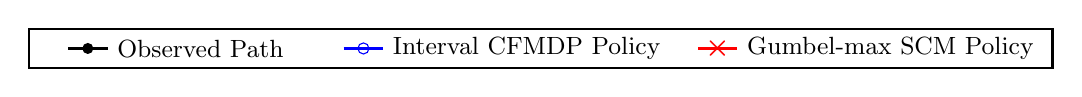
\begin{tikzpicture}[scale=1.0, every node/.style={scale=1.0}]
            \draw[thick, black] (-3, -0.25) rectangle (10, 0.25);
            %
            \draw[black, line width=1pt] (-2.5, 0.0) -- (-2,0.0);
            \fill[black] (-2.25,0.0) circle (2pt); %
            \node[right] at (-2,0.0) {\small Observed Path};
            
            %
            \draw[blue, line width=1pt] (1.0,0.0) -- (1.5,0.0);
            \node[draw=blue, circle, minimum size=4pt, inner sep=0pt] at (1.25,0.0) {}; %
            \node[right] at (1.5,0.0) {\small Interval CFMDP Policy};
            
            %
            \draw[red, line width=1pt] (5.5,0) -- (6,0);
            \node[red] at (5.75,0) {$\boldsymbol{\times}$}; %
            \node[right] at (6,0) {\small Gumbel-max SCM Policy};
        \end{tikzpicture}
    }\\
    %
    \subfigure[\footnotesize Lowest cumulative reward: Interval CFMDP ($312$), Gumbel-max SCM ($312$)]{%
        \resizebox{0.76\columnwidth}{!}{
             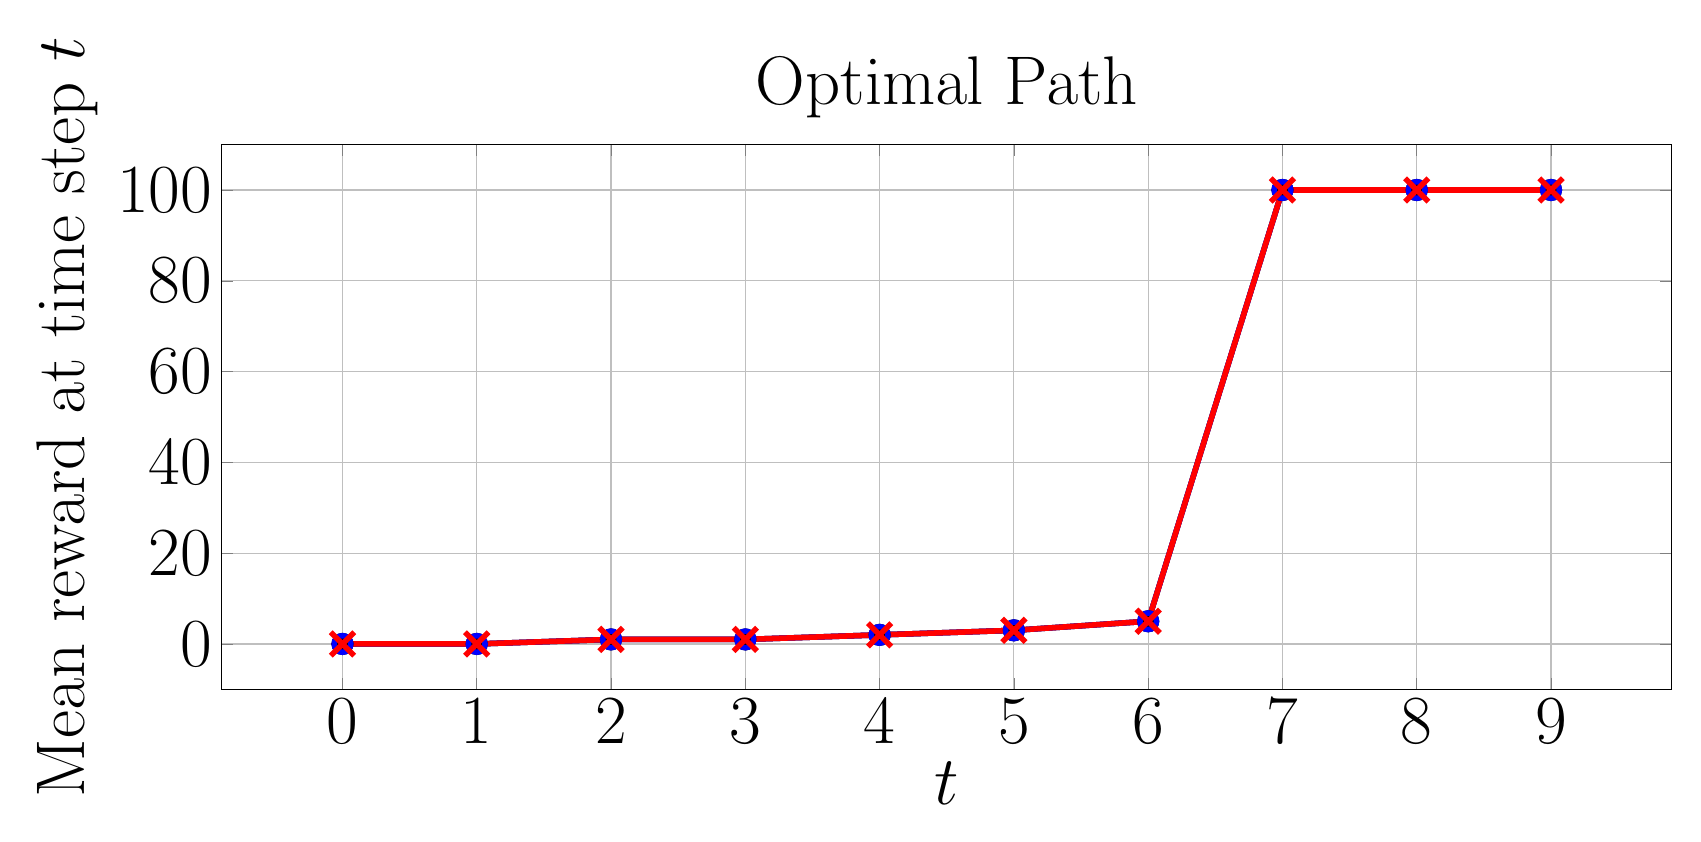
\begin{tikzpicture}
                \begin{axis}[
                    xlabel={$t$},
                    ylabel={Mean reward at time step $t$},
                    title={Optimal Path},
                    grid=both,
                    width=20cm, height=8.5cm,
                    every axis/.style={font=\Huge},
                    %
                ]
                \addplot[
                    color=black, %
                    mark=*, %
                    line width=2pt,
                    mark size=3pt,
                    error bars/.cd,
                    y dir=both, %
                    y explicit, %
                    error bar style={line width=1pt,solid},
                    error mark options={line width=1pt,mark size=4pt,rotate=90}
                ]
                coordinates {
                    (0, 0.0)  +- (0, 0.0)
                    (1, 0.0)  +- (0, 0.0) 
                    (2, 1.0)  +- (0, 0.0) 
                    (3, 1.0)  +- (0, 0.0)
                    (4, 2.0)  +- (0, 0.0)
                    (5, 3.0) +- (0, 0.0)
                    (6, 5.0) +- (0, 0.0)
                    (7, 100.0) +- (0, 0.0)
                    (8, 100.0) +- (0, 0.0)
                    (9, 100.0) +- (0, 0.0)
                };
                %
                \addplot[
                    color=blue, %
                    mark=o, %
                    line width=2pt,
                    mark size=3pt,
                    error bars/.cd,
                    y dir=both, %
                    y explicit, %
                    error bar style={line width=1pt,solid},
                    error mark options={line width=1pt,mark size=4pt,rotate=90}
                ]
                 coordinates {
                    (0, 0.0)  +- (0, 0.0)
                    (1, 0.0)  +- (0, 0.0) 
                    (2, 1.0)  +- (0, 0.0) 
                    (3, 1.0)  +- (0, 0.0)
                    (4, 2.0)  +- (0, 0.0)
                    (5, 3.0) +- (0, 0.0)
                    (6, 5.0) +- (0, 0.0)
                    (7, 100.0) +- (0, 0.0)
                    (8, 100.0) +- (0, 0.0)
                    (9, 100.0) +- (0, 0.0)
                };
                %
                \addplot[
                    color=red, %
                    mark=x, %
                    line width=2pt,
                    mark size=6pt,
                    error bars/.cd,
                    y dir=both, %
                    y explicit, %
                    error bar style={line width=1pt,solid},
                    error mark options={line width=1pt,mark size=4pt,rotate=90}
                ]
                coordinates {
                    (0, 0.0)  +- (0, 0.0)
                    (1, 0.0)  +- (0, 0.0) 
                    (2, 1.0)  +- (0, 0.0) 
                    (3, 1.0)  +- (0, 0.0)
                    (4, 2.0)  +- (0, 0.0)
                    (5, 3.0) +- (0, 0.0)
                    (6, 5.0) +- (0, 0.0)
                    (7, 100.0) +- (0, 0.0)
                    (8, 100.0) +- (0, 0.0)
                    (9, 100.0) +- (0, 0.0)
                };
                \end{axis}
            \end{tikzpicture}
         }
    }
    \hspace{1cm}
    \subfigure[\footnotesize Lowest cumulative reward: Interval CFMDP ($19$), Gumbel-max SCM ($-88$)]{%
         \resizebox{0.76\columnwidth}{!}{
            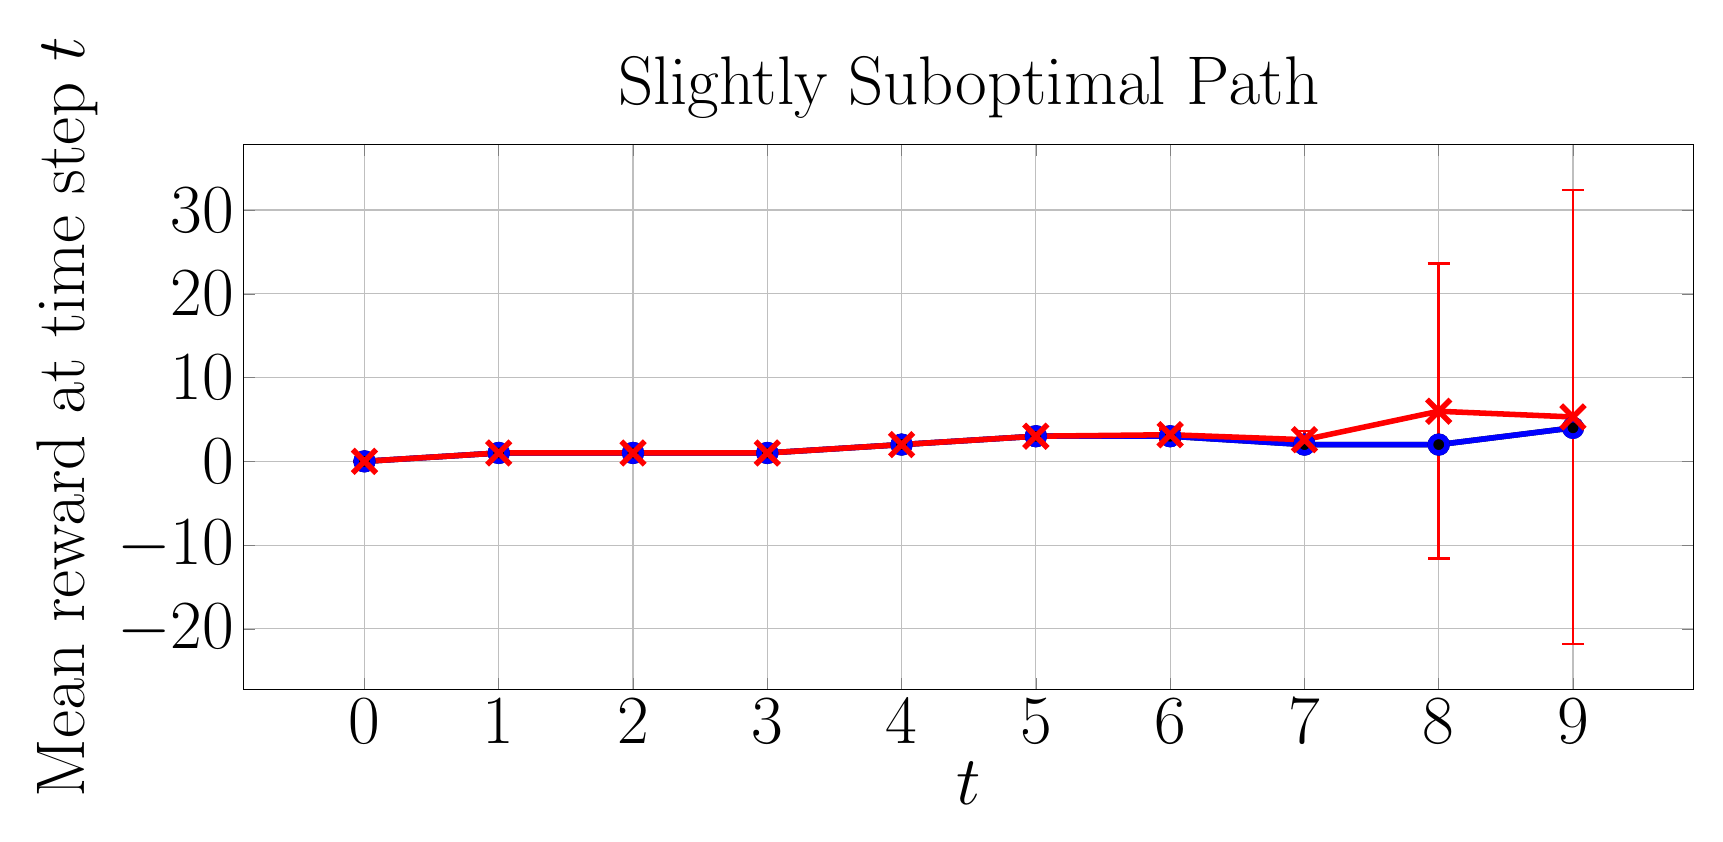
\begin{tikzpicture}
                \begin{axis}[
                    xlabel={$t$},
                    ylabel={Mean reward at time step $t$},
                    title={Slightly Suboptimal Path},
                    grid=both,
                    width=20cm, height=8.5cm,
                    every axis/.style={font=\Huge},
                    %
                ]
                \addplot[
                    color=black, %
                    mark=*, %
                    line width=2pt,
                    mark size=3pt,
                    error bars/.cd,
                    y dir=both, %
                    y explicit, %
                    error bar style={line width=1pt,solid},
                    error mark options={line width=1pt,mark size=4pt,rotate=90}
                ]
              coordinates {
                    (0, 0.0)  +- (0, 0.0)
                    (1, 1.0)  +- (0, 0.0) 
                    (2, 1.0)  +- (0, 0.0) 
                    (3, 1.0)  +- (0, 0.0)
                    (4, 2.0)  +- (0, 0.0)
                    (5, 3.0) +- (0, 0.0)
                    (6, 3.0) +- (0, 0.0)
                    (7, 2.0) +- (0, 0.0)
                    (8, 2.0) +- (0, 0.0)
                    (9, 4.0) +- (0, 0.0)
                };
                %
                \addplot[
                    color=blue, %
                    mark=o, %
                    line width=2pt,
                    mark size=3pt,
                    error bars/.cd,
                    y dir=both, %
                    y explicit, %
                    error bar style={line width=1pt,solid},
                    error mark options={line width=1pt,mark size=4pt,rotate=90}
                ]
              coordinates {
                    (0, 0.0)  +- (0, 0.0)
                    (1, 1.0)  +- (0, 0.0) 
                    (2, 1.0)  +- (0, 0.0) 
                    (3, 1.0)  +- (0, 0.0)
                    (4, 2.0)  +- (0, 0.0)
                    (5, 3.0) +- (0, 0.0)
                    (6, 3.0) +- (0, 0.0)
                    (7, 2.0) +- (0, 0.0)
                    (8, 2.0) +- (0, 0.0)
                    (9, 4.0) +- (0, 0.0)
                };
                %
                \addplot[
                    color=red, %
                    mark=x, %
                    line width=2pt,
                    mark size=6pt,
                    error bars/.cd,
                    y dir=both, %
                    y explicit, %
                    error bar style={line width=1pt,solid},
                    error mark options={line width=1pt,mark size=4pt,rotate=90}
                ]
                coordinates {
                    (0, 0.0)  +- (0, 0.0)
                    (1, 1.0)  +- (0, 0.0) 
                    (2, 1.0)  +- (0, 0.0) 
                    (3, 1.0)  +- (0, 0.0)
                    (4, 2.0)  += (0, 0.0)
                    (5, 3.0)  += (0, 0.0)
                    (6, 3.17847) += (0, 0.62606746) -= (0, 0.62606746)
                    (7, 2.5832885) += (0, 1.04598233) -= (0, 1.04598233)
                    (8, 5.978909) += (0, 17.60137623) -= (0, 17.60137623)
                    (9, 5.297059) += (0, 27.09227512) -= (0, 27.09227512)
                };
                \end{axis}
            \end{tikzpicture}
         }
    }\\[-1.5pt]
    \subfigure[\footnotesize Lowest cumulative reward: Interval CFMDP ($14$), Gumbel-max SCM ($-598$)]{%
         \resizebox{0.76\columnwidth}{!}{
             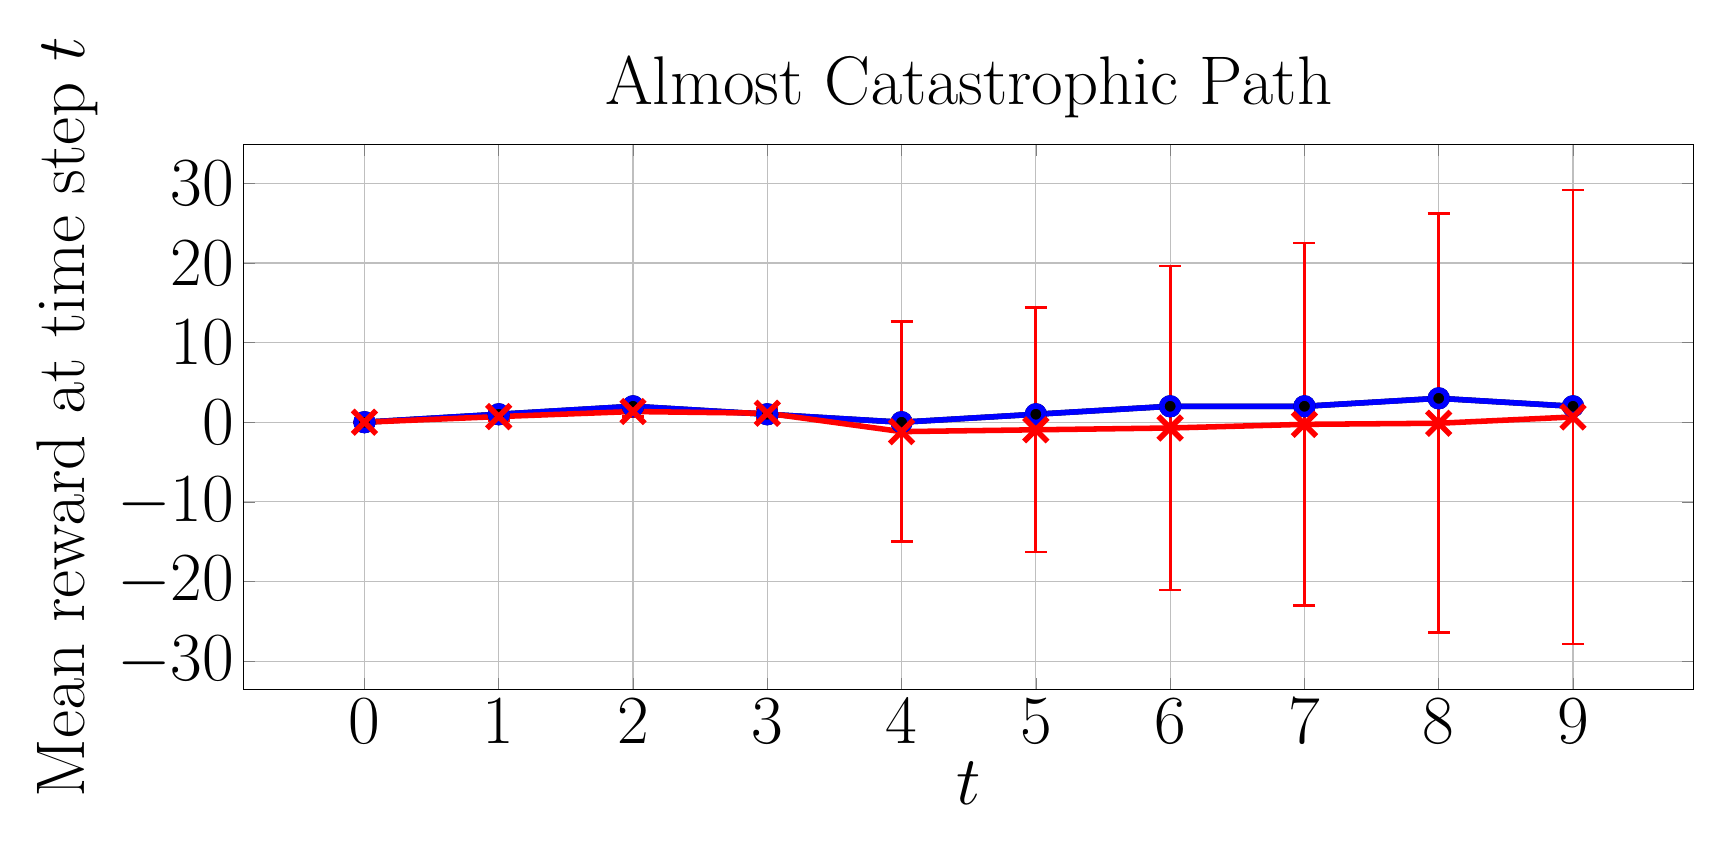
\begin{tikzpicture}
                \begin{axis}[
                    xlabel={$t$},
                    ylabel={Mean reward at time step $t$},
                    title={Almost Catastrophic Path},
                    grid=both,
                    width=20cm, height=8.5cm,
                    every axis/.style={font=\Huge},
                    %
                ]
                \addplot[
                    color=black, %
                    mark=*, %
                    line width=2pt,
                    mark size=3pt,
                    error bars/.cd,
                    y dir=both, %
                    y explicit, %
                    error bar style={line width=1pt,solid},
                    error mark options={line width=1pt,mark size=4pt,rotate=90}
                ]
                coordinates {
                    (0, 0.0)  +- (0, 0.0)
                    (1, 1.0)  +- (0, 0.0) 
                    (2, 2.0)  +- (0, 0.0) 
                    (3, 1.0)  +- (0, 0.0)
                    (4, 0.0)  +- (0, 0.0)
                    (5, 1.0) +- (0, 0.0)
                    (6, 2.0) +- (0, 0.0)
                    (7, 2.0) +- (0, 0.0)
                    (8, 3.0) +- (0, 0.0)
                    (9, 2.0) +- (0, 0.0)
                };
                %
                \addplot[
                    color=blue, %
                    mark=o, %
                    line width=2pt,
                    mark size=3pt,
                    error bars/.cd,
                    y dir=both, %
                    y explicit, %
                    error bar style={line width=1pt,solid},
                    error mark options={line width=1pt,mark size=4pt,rotate=90}
                ]
                coordinates {
                    (0, 0.0)  +- (0, 0.0)
                    (1, 1.0)  +- (0, 0.0) 
                    (2, 2.0)  +- (0, 0.0) 
                    (3, 1.0)  +- (0, 0.0)
                    (4, 0.0)  +- (0, 0.0)
                    (5, 1.0) +- (0, 0.0)
                    (6, 2.0) +- (0, 0.0)
                    (7, 2.0) +- (0, 0.0)
                    (8, 3.0) +- (0, 0.0)
                    (9, 2.0) +- (0, 0.0)
                };
                %
                \addplot[
                    color=red, %
                    mark=x, %
                    line width=2pt,
                    mark size=6pt,
                    error bars/.cd,
                    y dir=both, %
                    y explicit, %
                    error bar style={line width=1pt,solid},
                    error mark options={line width=1pt,mark size=4pt,rotate=90}
                ]
                coordinates {
                    (0, 0.0)  +- (0, 0.0)
                    (1, 0.7065655)  +- (0, 0.4553358) 
                    (2, 1.341673)  +- (0, 0.67091621) 
                    (3, 1.122926)  +- (0, 0.61281824)
                    (4, -1.1821935)  +- (0, 13.82444042)
                    (5, -0.952399)  +- (0, 15.35195457)
                    (6, -0.72672) +- (0, 20.33508414)
                    (7, -0.268983) +- (0, 22.77861454)
                    (8, -0.1310835) +- (0, 26.31013314)
                    (9, 0.65806) +- (0, 28.50670214)
                };
                %
            %
            %
            %
            %
            %
            %
            %
            %
            %
            %
            %
            %
            %
            %
            %
            %
            %
            %
                \end{axis}
            \end{tikzpicture}
         }
    }
    \hspace{1cm}
    \subfigure[\footnotesize Lowest cumulative reward: Interval CFMDP ($-698$), Gumbel-max SCM ($-698$)]{%
         \resizebox{0.76\columnwidth}{!}{
            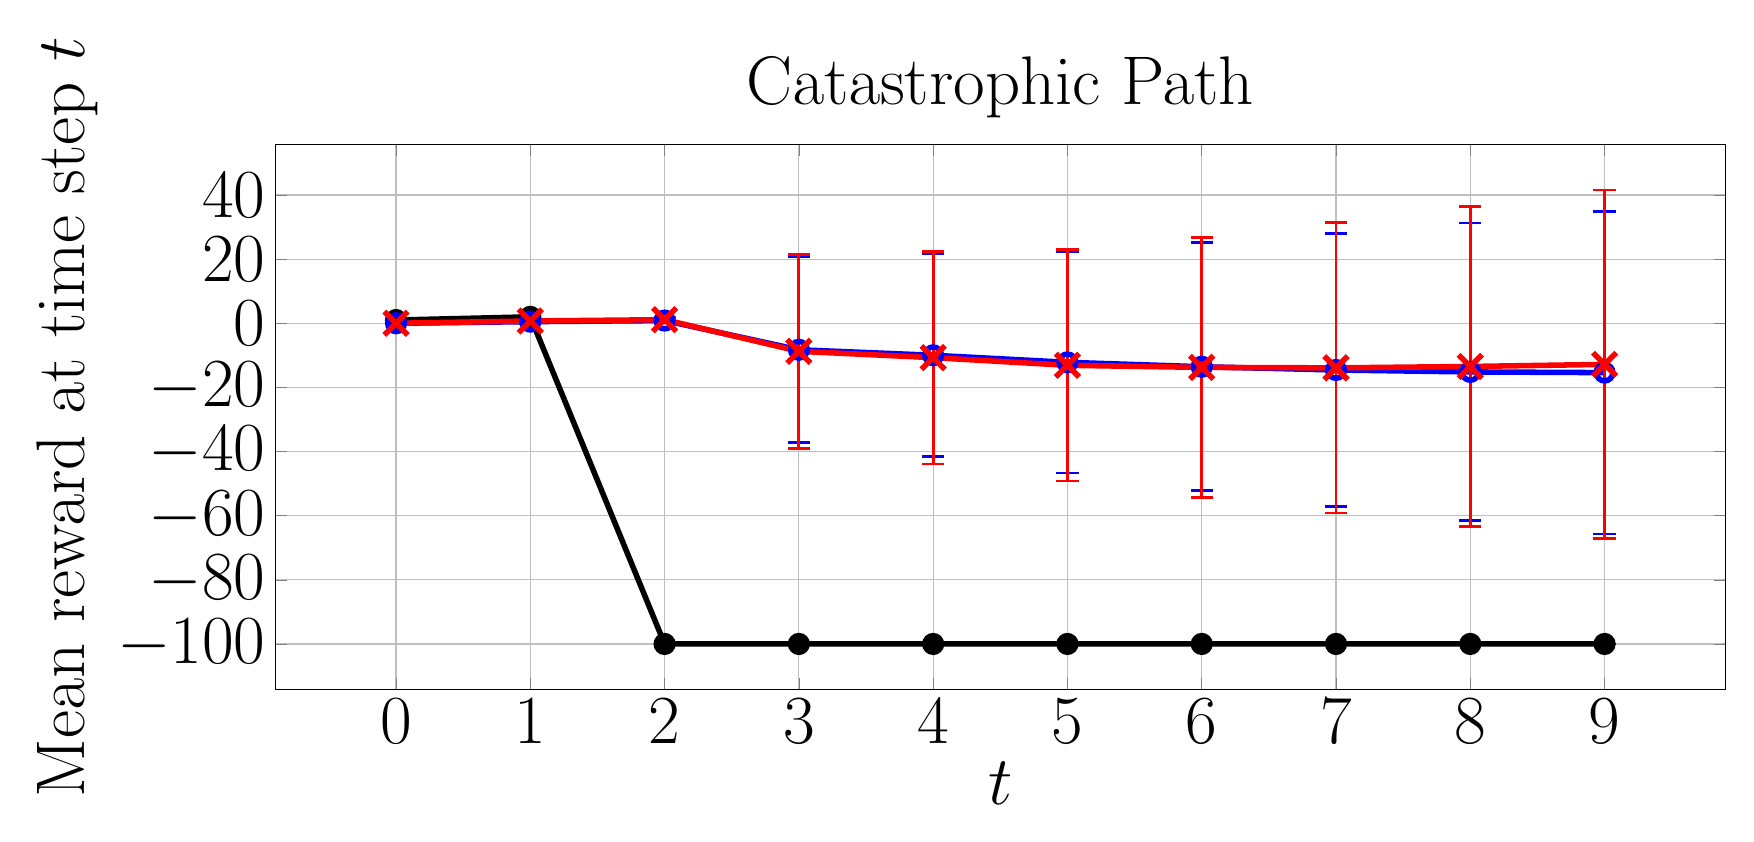
\begin{tikzpicture}
                \begin{axis}[
                    xlabel={$t$},
                    ylabel={Mean reward at time step $t$},
                    title={Catastrophic Path},
                    grid=both,
                    width=20cm, height=8.5cm,
                    every axis/.style={font=\Huge},
                    %
                ]
                \addplot[
                    color=black, %
                    mark=*, %
                    line width=2pt,
                    mark size=3pt,
                    error bars/.cd,
                    y dir=both, %
                    y explicit, %
                    error bar style={line width=1pt,solid},
                    error mark options={line width=1pt,mark size=4pt,rotate=90}
                ]
                coordinates {
                    (0, 1.0)  +- (0, 0.0)
                    (1, 2.0)  +- (0, 0.0) 
                    (2, -100.0)  +- (0, 0.0) 
                    (3, -100.0)  +- (0, 0.0)
                    (4, -100.0)  +- (0, 0.0)
                    (5, -100.0) +- (0, 0.0)
                    (6, -100.0) +- (0, 0.0)
                    (7, -100.0) +- (0, 0.0)
                    (8, -100.0) +- (0, 0.0)
                    (9, -100.0) +- (0, 0.0)
                };
                %
                \addplot[
                    color=blue, %
                    mark=o, %
                    line width=2pt,
                    mark size=3pt,
                    error bars/.cd,
                    y dir=both, %
                    y explicit, %
                    error bar style={line width=1pt,solid},
                    error mark options={line width=1pt,mark size=4pt,rotate=90}
                ]
                coordinates {
                    (0, 0.0)  +- (0, 0.0)
                    (1, 0.504814)  +- (0, 0.49997682) 
                    (2, 0.8439835)  +- (0, 0.76831917) 
                    (3, -8.2709165)  +- (0, 28.93656754)
                    (4, -9.981082)  +- (0, 31.66825363)
                    (5, -12.1776325) +- (0, 34.53463233)
                    (6, -13.556076) +- (0, 38.62845372)
                    (7, -14.574418) +- (0, 42.49603359)
                    (8, -15.1757075) +- (0, 46.41913968)
                    (9, -15.3900395) +- (0, 50.33563368)
                };
                %
                \addplot[
                    color=red, %
                    mark=x, %
                    line width=2pt,
                    mark size=6pt,
                    error bars/.cd,
                    y dir=both, %
                    y explicit, %
                    error bar style={line width=1pt,solid},
                    error mark options={line width=1pt,mark size=4pt,rotate=90}
                ]
                coordinates {
                    (0, 0.0)  +- (0, 0.0)
                    (1, 0.701873)  +- (0, 0.45743556) 
                    (2, 1.1227805)  +- (0, 0.73433129) 
                    (3, -8.7503255)  +- (0, 30.30257976)
                    (4, -10.722092)  +- (0, 33.17618589)
                    (5, -13.10721)  +- (0, 36.0648089)
                    (6, -13.7631645) +- (0, 40.56553451)
                    (7, -13.909043) +- (0, 45.23829402)
                    (8, -13.472517) +- (0, 49.96270296)
                    (9, -12.8278835) +- (0, 54.38618735)
                };
                %
            %
            %
            %
            %
            %
            %
            %
            %
            %
            %
            %
            %
            %
            %
            %
            %
            %
            %
                \end{axis}
            \end{tikzpicture}
         }
    }
    \caption{Average instant reward of CF paths induced by policies on GridWorld $p=0.4$.}
    \label{fig: reward p=0.4}
\end{figure*}

\subsection{Experimental Setup}
To compare policy performance, we measure the average rewards of counterfactual paths induced by our policy and the Gumbel-max policy by uniformly sampling $200$ counterfactual MDPs from the ICFMDP and generating $10,000$ counterfactual paths over each sampled CFMDP. \jl{Since the interval CFMDP depends on the observed path, we select $4$  paths of varying optimality to evaluate how the observed path impacts the performance of both policies: an optimal path, a slightly suboptimal path that could reach the optimal reward with a few changes, a catastrophic path that enters a catastrophic, terminal state with low reward, and an almost catastrophic path that was close to entering a catastrophic state.} When measuring the average probability bound widths and execution time needed to generate the ICFMDPs, we averaged over $20$ randomly generated observed paths
\footnote{Further training details are provided in Appendix \ref{app: training details}, and the code is provided at \href{https://github.com/ddv-lab/robust-cf-inference-in-MDPs}{https://github.com/ddv-lab/robust-cf-inference-in-MDPs}
%
%
.}.

\subsection{GridWorld}
\jl{The GridWorld MDP is a $4 \times 4$ grid where an agent must navigate from the top-left corner to the goal state in the bottom-right corner, avoiding a dangerous terminal state in the centre. At each time step, the agent can move up, down, left, or right, but there is a small probability (controlled by hyper-parameter $p$) of moving in an unintended direction. As the agent nears the goal, the reward for each state increases, culminating in a reward of $+100$ for reaching the goal. Entering the dangerous state results in a penalty of $-100$. We use two versions of GridWorld: a less stochastic version with $p=0.9$ (i.e., $90$\% chance of moving in the chosen direction) and a more stochastic version with $p=0.4$.}

\paragraph{GridWorld ($p=0.9$)}
When $p=0.9$, the counterfactual probability bounds are typically narrow (see Table \ref{tab:nonzero_probs} for average measurements). Consequently, as shown in Figure \ref{fig: reward p=0.9}, both policies are nearly identical and perform similarly well across the optimal, slightly suboptimal, and catastrophic paths.
%
However, for the almost catastrophic path, the interval CFMDP path is more conservative and follows the observed path more closely (as this is where the probability bounds are narrowest), which typically requires one additional step to reach the goal state than the Gumbel-max SCM policy.
%

\paragraph{GridWorld ($p=0.4$)}
\jl{When $p=0.4$, the GridWorld environment becomes more uncertain, increasing the risk of entering the dangerous state even if correct actions are chosen. Thus, as shown in Figure \ref{fig: reward p=0.4}, the interval CFMDP policy adopts a more conservative approach, avoiding deviation from the observed policy if it cannot guarantee higher counterfactual rewards (see the slightly suboptimal and almost catastrophic paths), whereas the Gumbel-max SCM is inconsistent: it can yield higher rewards, but also much lower rewards, reflected in the wide error bars.} For the catastrophic path, both policies must deviate from the observed path to achieve a higher reward and, in this case, perform similarly.
%
%
%
%
\subsection{Sepsis}
The Sepsis MDP \citep{oberst2019counterfactual} simulates trajectories of Sepsis patients. Each state consists of four vital signs (heart rate, blood pressure, oxygen concentration, and glucose levels), categorised as low, normal, or high.
and three treatments that can be toggled on/off at each time step (8 actions in total). Unlike \citet{oberst2019counterfactual}, we scale rewards based on the number of out-of-range vital signs, between $-1000$ (patient dies) and $1000$ (patient discharged). \jl{Like the GridWorld $p=0.4$ experiment, the Sepsis MDP is highly uncertain, as many states are equally likely to lead to optimal and poor outcomes. Thus, as shown in Figure \ref{fig: reward sepsis}, both policies follow the observed optimal and almost catastrophic paths to guarantee rewards are no worse than the observation.} However, improving the catastrophic path requires deviating from the observation. Here, the Gumbel-max SCM policy, on average, performs better than the interval CFMDP policy. But, since both policies have lower bounds clipped at $-1000$, neither policy reliably improves over the observation. In contrast, for the slightly suboptimal path, the interval CFMDP policy performs significantly better, shown by its higher lower bounds. 
Moreover, in these two cases, the worst-case counterfactual path generated by the interval CFMDP policy is better than that of the Gumbel-max SCM policy,
indicating its greater robustness.
%
\begin{figure*}
    \centering
     \resizebox{0.6\textwidth}{!}{
        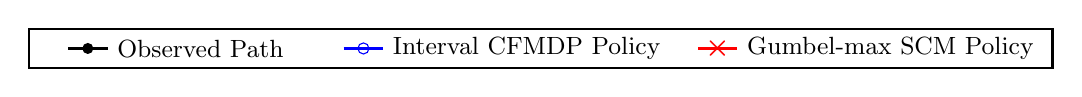
\begin{tikzpicture}[scale=1.0, every node/.style={scale=1.0}]
            \draw[thick, black] (-3, -0.25) rectangle (10, 0.25);
            %
            \draw[black, line width=1pt] (-2.5, 0.0) -- (-2,0.0);
            \fill[black] (-2.25,0.0) circle (2pt); %
            \node[right] at (-2,0.0) {\small Observed Path};
            
            %
            \draw[blue, line width=1pt] (1.0,0.0) -- (1.5,0.0);
            \node[draw=blue, circle, minimum size=4pt, inner sep=0pt] at (1.25,0.0) {}; %
            \node[right] at (1.5,0.0) {\small Interval CFMDP Policy};
            
            %
            \draw[red, line width=1pt] (5.5,0) -- (6,0);
            \node[red] at (5.75,0) {$\boldsymbol{\times}$}; %
            \node[right] at (6,0) {\small Gumbel-max SCM Policy};
        \end{tikzpicture}
    }\\
    \subfigure[\footnotesize Lowest cumulative reward: Interval CFMDP ($8000$), Gumbel-max SCM ($8000$)]{%
         \resizebox{0.76\columnwidth}{!}{
             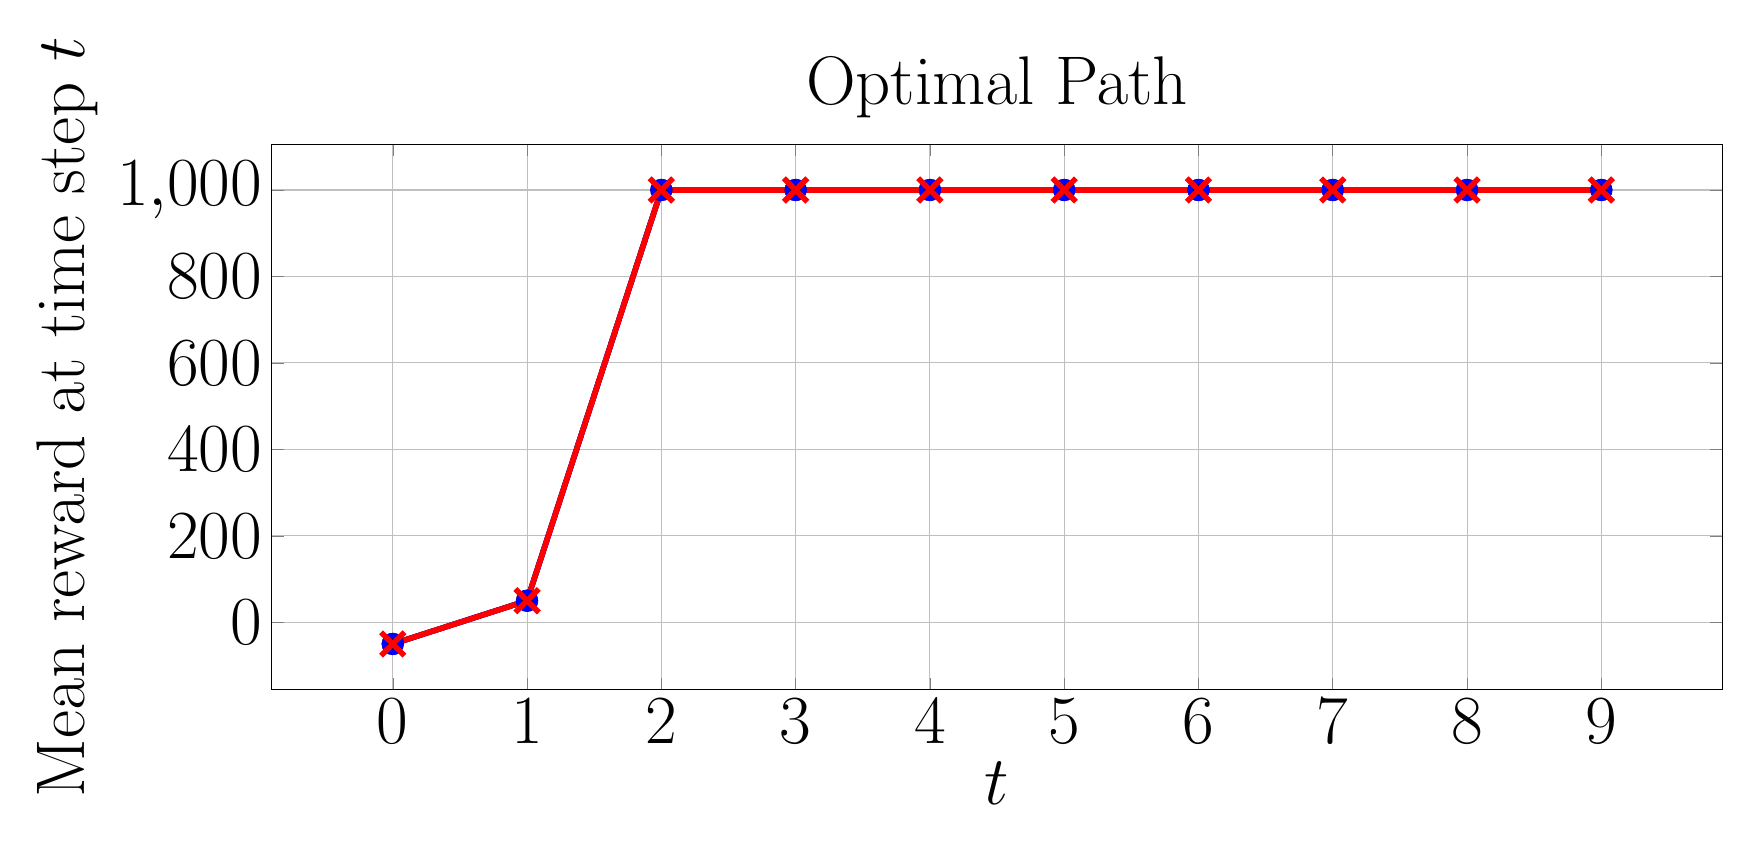
\begin{tikzpicture}
                \begin{axis}[
                    xlabel={$t$},
                    ylabel={Mean reward at time step $t$},
                    title={Optimal Path},
                    grid=both,
                    width=20cm, height=8.5cm,
                    every axis/.style={font=\Huge},
                    %
                ]
                \addplot[
                    color=black, %
                    mark=*, %
                    line width=2pt,
                    mark size=3pt,
                ]
                coordinates {
                    (0, -50.0)
                    (1, 50.0)
                    (2, 1000.0)
                    (3, 1000.0)
                    (4, 1000.0)
                    (5, 1000.0)
                    (6, 1000.0)
                    (7, 1000.0)
                    (8, 1000.0)
                    (9, 1000.0)
                };
                %
                \addplot[
                    color=blue, %
                    mark=o, %
                    line width=2pt,
                    mark size=3pt,
                    error bars/.cd,
                    y dir=both, %
                    y explicit, %
                    error bar style={line width=1pt,solid},
                    error mark options={line width=1pt,mark size=4pt,rotate=90}
                ]
                coordinates {
                    (0, -50.0)  +- (0, 0.0)
                    (1, 50.0)  +- (0, 0.0) 
                    (2, 1000.0)  +- (0, 0.0) 
                    (3, 1000.0)  +- (0, 0.0)
                    (4, 1000.0)  +- (0, 0.0)
                    (5, 1000.0) +- (0, 0.0)
                    (6, 1000.0) +- (0, 0.0)
                    (7, 1000.0) +- (0, 0.0)
                    (8, 1000.0) +- (0, 0.0)
                    (9, 1000.0) +- (0, 0.0)
                };
                %
                \addplot[
                    color=red, %
                    mark=x, %
                    line width=2pt,
                    mark size=6pt,
                    error bars/.cd,
                    y dir=both, %
                    y explicit, %
                    error bar style={line width=1pt,solid},
                    error mark options={line width=1pt,mark size=4pt,rotate=90}
                ]
                coordinates {
                    (0, -50.0)  +- (0, 0.0)
                    (1, 50.0)  +- (0, 0.0) 
                    (2, 1000.0)  +- (0, 0.0) 
                    (3, 1000.0)  +- (0, 0.0)
                    (4, 1000.0)  +- (0, 0.0)
                    (5, 1000.0) +- (0, 0.0)
                    (6, 1000.0) +- (0, 0.0)
                    (7, 1000.0) +- (0, 0.0)
                    (8, 1000.0) +- (0, 0.0)
                    (9, 1000.0) +- (0, 0.0)
                };
                %
                \end{axis}
            \end{tikzpicture}
         }
    }
    \hspace{1cm}
    \subfigure[\footnotesize Lowest cumulative reward: Interval CFMDP ($-5980$), Gumbel-max SCM ($-8000$)]{%
         \resizebox{0.76\columnwidth}{!}{
            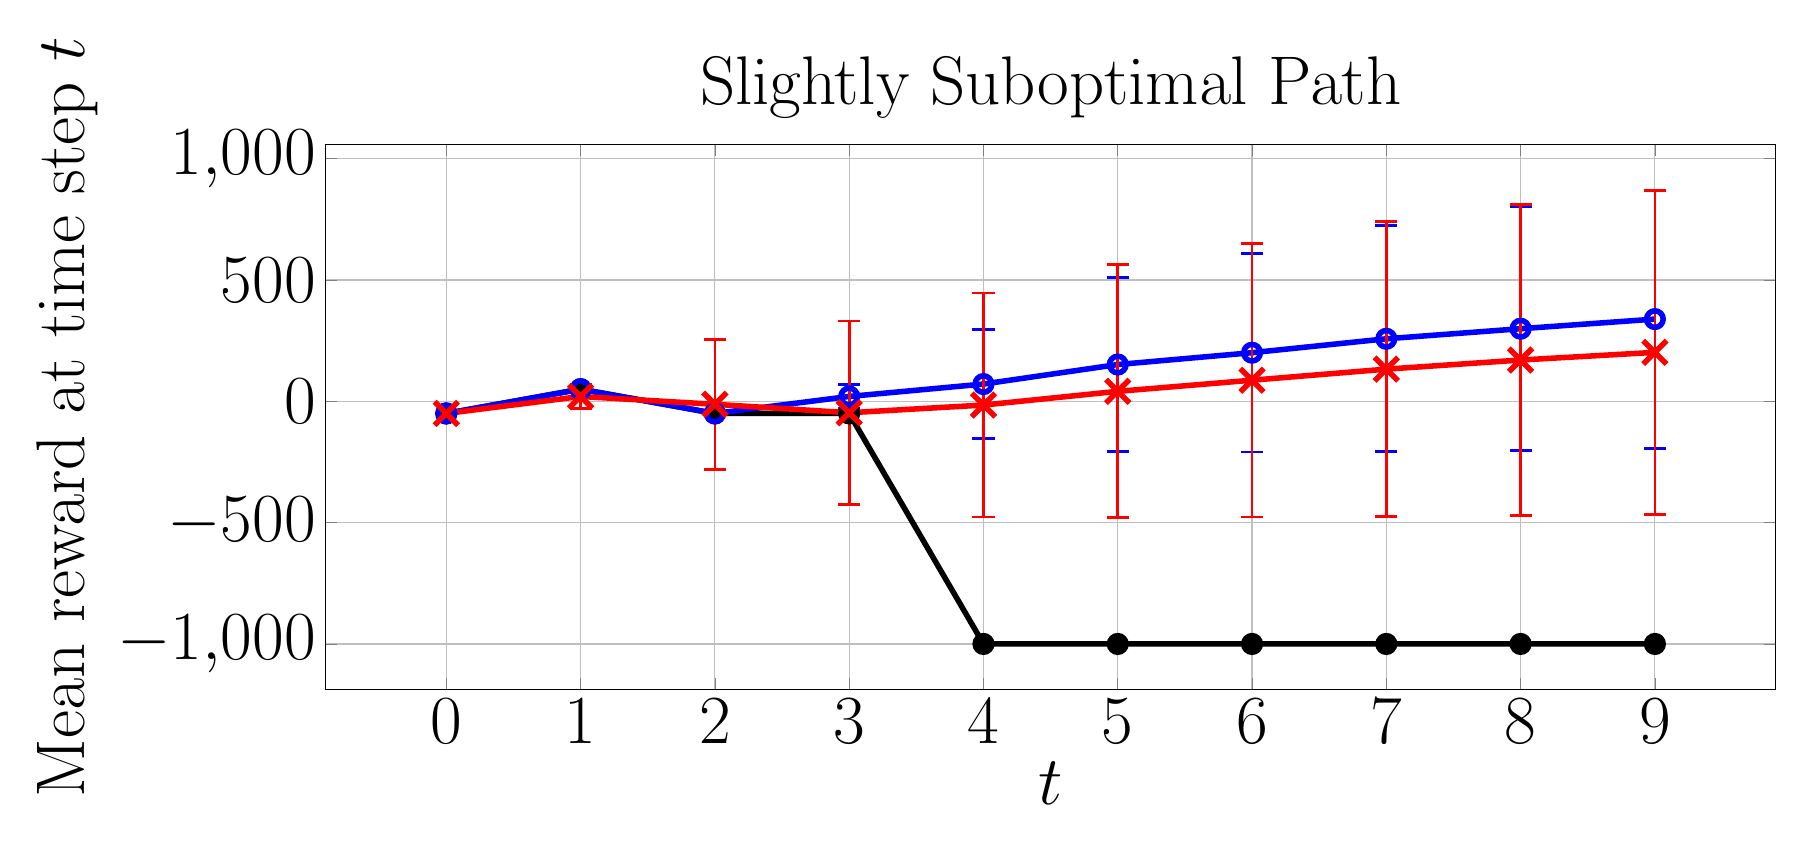
\begin{tikzpicture}
                \begin{axis}[
                    xlabel={$t$},
                    ylabel={Mean reward at time step $t$},
                    title={Slightly Suboptimal Path},
                    grid=both,
                    width=20cm, height=8.5cm,
                    every axis/.style={font=\Huge},
                    %
                ]
               \addplot[
                    color=black, %
                    mark=*, %
                    line width=2pt,
                    mark size=3pt,
                ]
                coordinates {
                    (0, -50.0)
                    (1, 50.0)
                    (2, -50.0)
                    (3, -50.0)
                    (4, -1000.0)
                    (5, -1000.0)
                    (6, -1000.0)
                    (7, -1000.0)
                    (8, -1000.0)
                    (9, -1000.0)
                };
                %
                \addplot[
                    color=blue, %
                    mark=o, %
                    line width=2pt,
                    mark size=3pt,
                    error bars/.cd,
                    y dir=both, %
                    y explicit, %
                    error bar style={line width=1pt,solid},
                    error mark options={line width=1pt,mark size=4pt,rotate=90}
                ]
                coordinates {
                    (0, -50.0)  +- (0, 0.0)
                    (1, 50.0)  +- (0, 0.0) 
                    (2, -50.0)  +- (0, 0.0) 
                    (3, 20.0631)  +- (0, 49.97539413)
                    (4, 71.206585)  +- (0, 226.02033693)
                    (5, 151.60797) +- (0, 359.23292559)
                    (6, 200.40593) +- (0, 408.86185176)
                    (7, 257.77948) +- (0, 466.10372804)
                    (8, 299.237465) +- (0, 501.82579506)
                    (9, 338.9129) +- (0, 532.06124996)
                };
                %
                \addplot[
                    color=red, %
                    mark=x, %
                    line width=2pt,
                    mark size=6pt,
                    error bars/.cd,
                    y dir=both, %
                    y explicit, %
                    error bar style={line width=1pt,solid},
                    error mark options={line width=1pt,mark size=4pt,rotate=90}
                ]
                coordinates {
                    (0, -50.0)  +- (0, 0.0)
                    (1, 20.00736)  +- (0, 49.99786741) 
                    (2, -12.282865)  +- (0, 267.598755) 
                    (3, -47.125995)  +- (0, 378.41755832)
                    (4, -15.381965)  +- (0, 461.77616558)
                    (5, 41.15459) +- (0, 521.53189262)
                    (6, 87.01595) +- (0, 564.22243126 )
                    (7, 132.62376) +- (0, 607.31338037)
                    (8, 170.168145) +- (0, 641.48013693)
                    (9, 201.813135) +- (0, 667.29441777)
                };
                %
                %
                %
                %
                %
                %
                %
                %
                %
                %
                %
                %
                %
                %
                %
                %
                %
                %
                %
                \end{axis}
            \end{tikzpicture}
         }
    }\\[-1.5pt]
    \subfigure[\footnotesize Lowest cumulative reward: Interval CFMDP ($100$), Gumbel-max SCM ($100$)]{%
         \resizebox{0.76\columnwidth}{!}{
             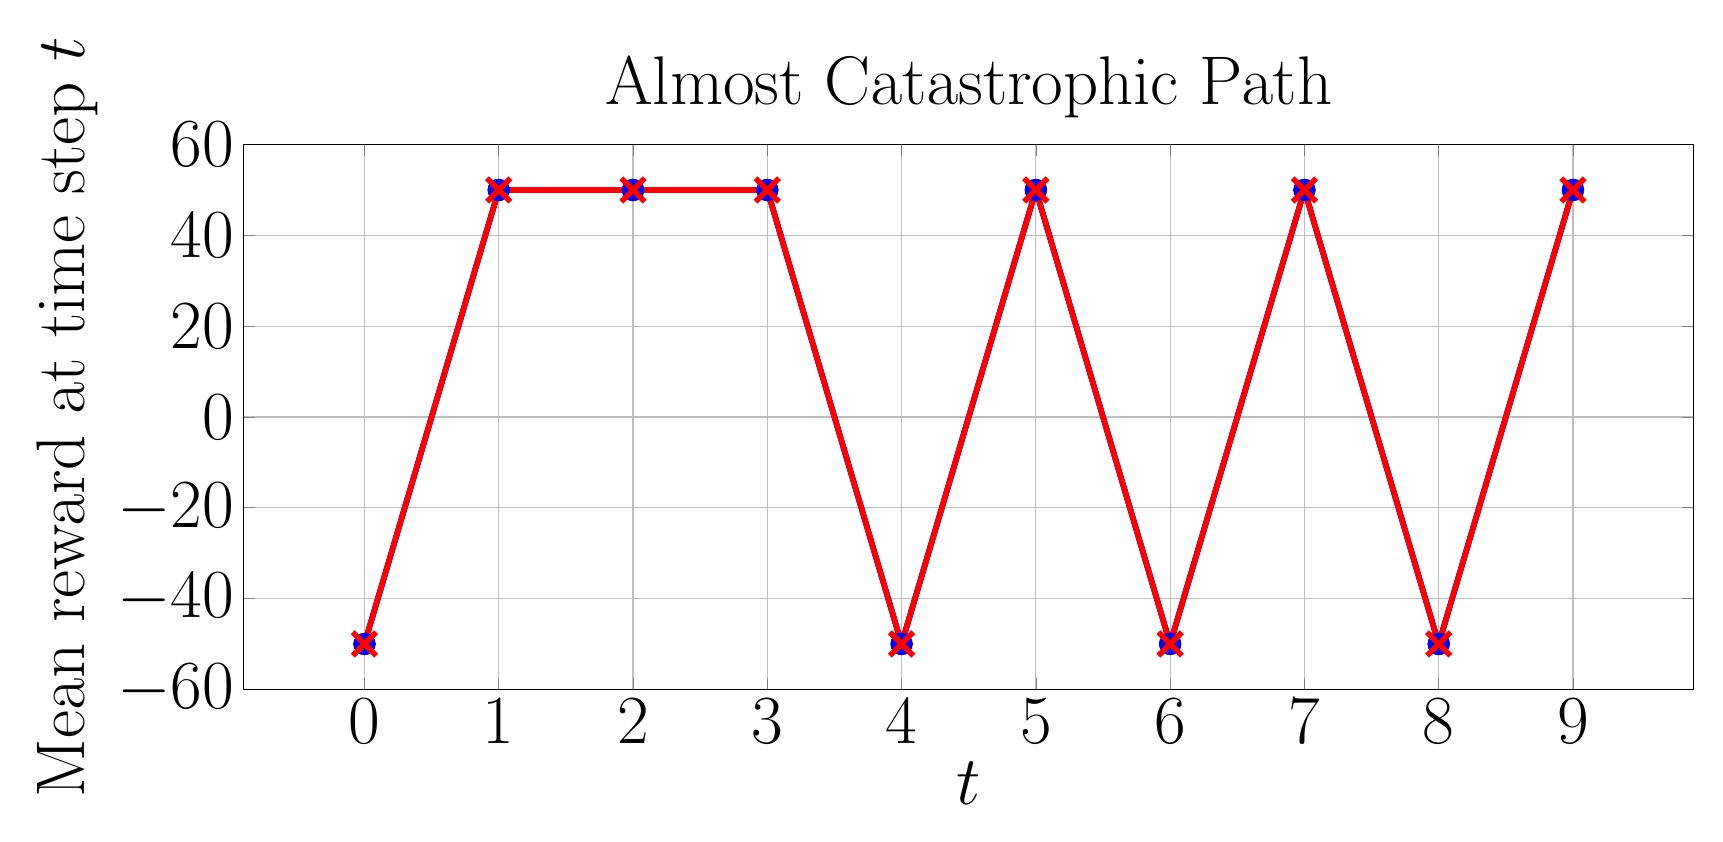
\begin{tikzpicture}
                \begin{axis}[
                    xlabel={$t$},
                    ylabel={Mean reward at time step $t$},
                    title={Almost Catastrophic Path},
                    grid=both,
                    every axis/.style={font=\Huge},
                    width=20cm, height=8.5cm,
                    %
                ]
               \addplot[
                    color=black, %
                    mark=*, %
                    line width=2pt,
                    mark size=3pt,
                ]
                coordinates {
                    (0, -50.0)
                    (1, 50.0)
                    (2, 50.0)
                    (3, 50.0)
                    (4, -50.0)
                    (5, 50.0)
                    (6, -50.0)
                    (7, 50.0)
                    (8, -50.0)
                    (9, 50.0)
                };
                %
                %
                \addplot[
                    color=blue, %
                    mark=o, %
                    line width=2pt,
                    mark size=3pt,
                    error bars/.cd,
                    y dir=both, %
                    y explicit, %
                    error bar style={line width=1pt,solid},
                    error mark options={line width=1pt,mark size=4pt,rotate=90}
                ]
                coordinates {
                    (0, -50.0)  +- (0, 0.0)
                    (1, 50.0)  +- (0, 0.0) 
                    (2, 50.0)  +- (0, 0.0) 
                    (3, 50.0)  +- (0, 0.0)
                    (4, -50.0)  +- (0, 0.0)
                    (5, 50.0) +- (0, 0.0)
                    (6, -50.0) +- (0, 0.0)
                    (7, 50.0) +- (0, 0.0)
                    (8, -50.0) +- (0, 0.0)
                    (9, 50.0) +- (0, 0.0)
                };
                %
                \addplot[
                    color=red, %
                    mark=x, %
                    line width=2pt,
                    mark size=6pt,
                    error bars/.cd,
                    y dir=both, %
                    y explicit, %
                    error bar style={line width=1pt,solid},
                    error mark options={line width=1pt,mark size=4pt,rotate=90}
                ]
                coordinates {
                    (0, -50.0)  +- (0, 0.0)
                    (1, 50.0)  +- (0, 0.0) 
                    (2, 50.0)  +- (0, 0.0) 
                    (3, 50.0)  +- (0, 0.0)
                    (4, -50.0)  +- (0, 0.0)
                    (5, 50.0) +- (0, 0.0)
                    (6, -50.0) +- (0, 0.0)
                    (7, 50.0) +- (0, 0.0)
                    (8, -50.0) +- (0, 0.0)
                    (9, 50.0) +- (0, 0.0)
                };
                %
                %
                %
                %
                %
                %
                %
                %
                %
                %
                %
                %
                %
                %
                %
                %
                %
                %
                %
                \end{axis}
            \end{tikzpicture}
         }
    }
    \hspace{1cm}
    \subfigure[\footnotesize Lowest cumulative reward: Interval CFMDP ($-7150$), Gumbel-max SCM ($-9050$)]{%
         \resizebox{0.76\columnwidth}{!}{
            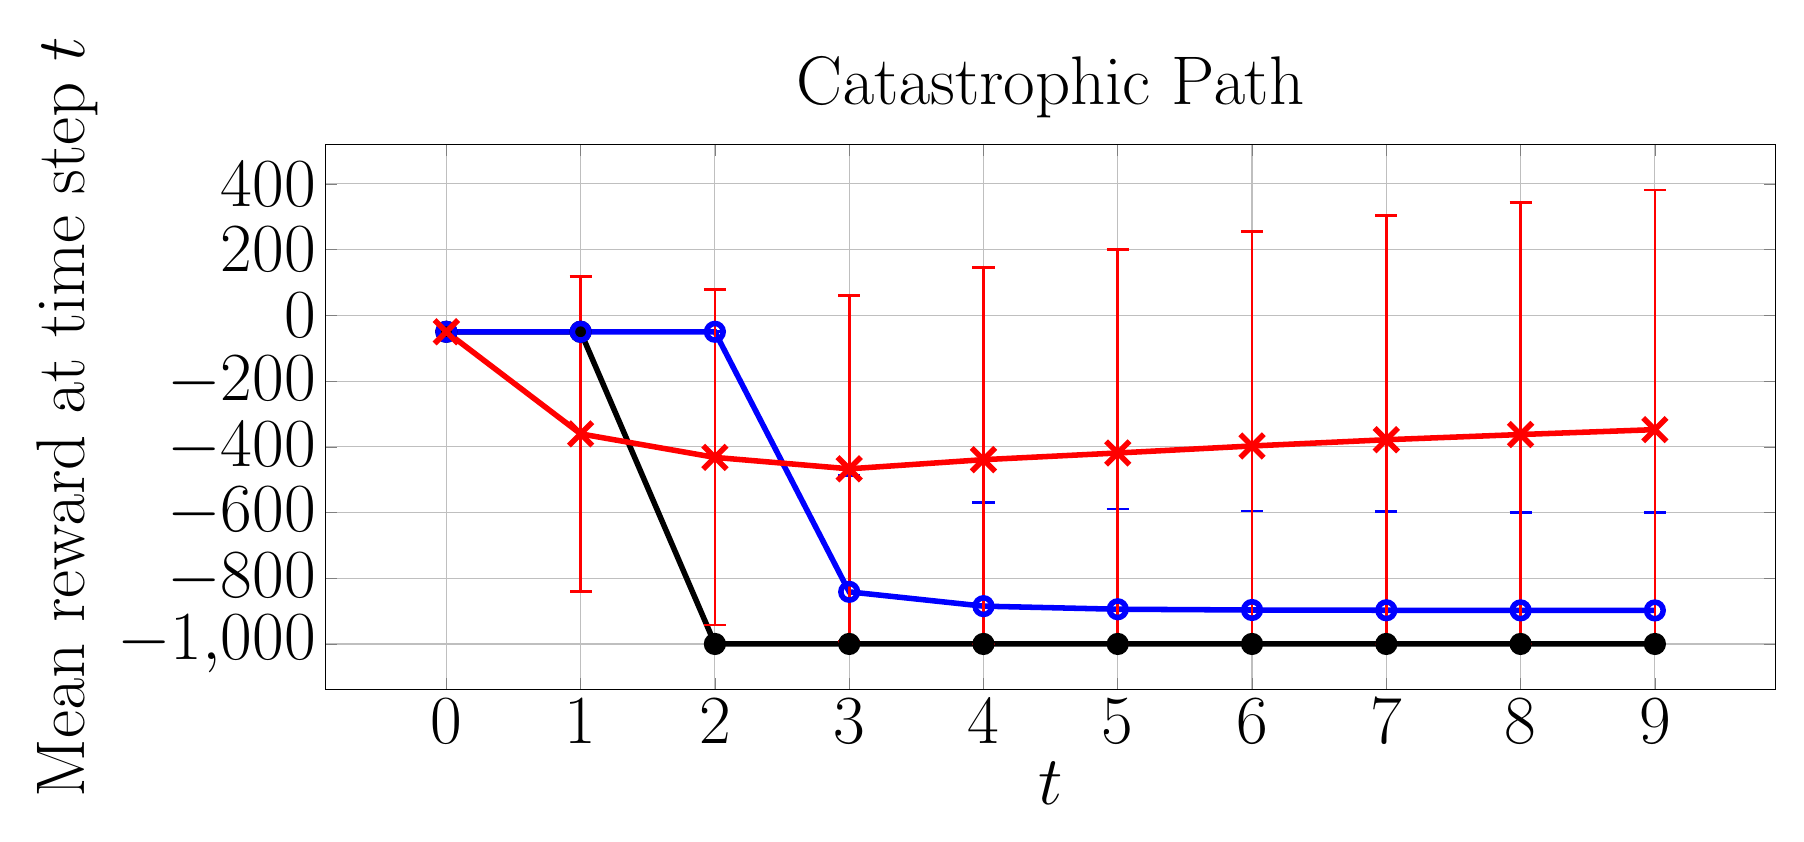
\begin{tikzpicture}
                \begin{axis}[
                    xlabel={$t$},
                    ylabel={Mean reward at time step $t$},
                    title={Catastrophic Path},
                    grid=both,
                    width=20cm, height=8.5cm,
                    every axis/.style={font=\Huge},
                    %
                ]
               \addplot[
                    color=black, %
                    mark=*, %
                    line width=2pt,
                    mark size=3pt,
                ]
                coordinates {
                    (0, -50.0)
                    (1, -50.0)
                    (2, -1000.0)
                    (3, -1000.0)
                    (4, -1000.0)
                    (5, -1000.0)
                    (6, -1000.0)
                    (7, -1000.0)
                    (8, -1000.0)
                    (9, -1000.0)
                };
                %
                %
                \addplot[
                    color=blue, %
                    mark=o, %
                    line width=2pt,
                    mark size=3pt,
                    error bars/.cd,
                    y dir=both, %
                    y explicit, %
                    error bar style={line width=1pt,solid},
                    error mark options={line width=1pt,mark size=4pt,rotate=90}
                ]
                coordinates {
                    (0, -50.0)  +- (0, 0.0)
                    (1, -50.0)  +- (0, 0.0) 
                    (2, -50.0)  +- (0, 0.0) 
                    (3, -841.440725)  += (0, 354.24605512) -= (0, 158.559275)
                    (4, -884.98225)  += (0, 315.37519669) -= (0, 115.01775)
                    (5, -894.330425) += (0, 304.88572805) -= (0, 105.669575)
                    (6, -896.696175) += (0, 301.19954514) -= (0, 103.303825)
                    (7, -897.4635) += (0, 299.61791279) -= (0, 102.5365)
                    (8, -897.77595) += (0, 298.80392585) -= (0, 102.22405)
                    (9, -897.942975) += (0, 298.32920557) -= (0, 102.057025)
                };
                %
                \addplot[
                    color=red, %
                    mark=x, %
                    line width=2pt,
                    mark size=6pt,
                    error bars/.cd,
                    y dir=both, %
                    y explicit, %
                    error bar style={line width=1pt,solid},
                    error mark options={line width=1pt,mark size=4pt,rotate=90}
                ]
            coordinates {
                    (0, -50.0)  +- (0, 0.0)
                    (1, -360.675265)  +- (0, 479.39812699) 
                    (2, -432.27629)  +- (0, 510.38620897) 
                    (3, -467.029545)  += (0, 526.36009628) -= (0, 526.36009628)
                    (4, -439.17429)  += (0, 583.96638919) -= (0, 560.82571)
                    (5, -418.82704) += (0, 618.43027478) -= (0, 581.17296)
                    (6, -397.464895) += (0, 652.67322574) -= (0, 602.535105)
                    (7, -378.49052) += (0, 682.85407033) -= (0, 621.50948)
                    (8, -362.654195) += (0, 707.01412023) -= (0, 637.345805)
                    (9, -347.737935) += (0, 729.29076479) -= (0, 652.262065)
                };
                %
                %
                %
                %
                %
                %
                %
                %
                %
                %
                %
                %
                %
                %
                %
                %
                %
                %
                %
                \end{axis}
            \end{tikzpicture}
         }
    }
    \caption{Average instant reward of CF paths induced by policies on Sepsis.}
    \label{fig: reward sepsis}
\end{figure*}

%
%
%
\subsection{Interval CFMDP Bounds}
%
%
Table \ref{tab:nonzero_probs} presents the mean counterfactual probability bound widths (excluding transitions where the upper bound is $0$) for each MDP, averaged over 20 observed paths. We compare the bounds under counterfactual stability (CS) and monotonicity (M) assumptions, CS alone, and no assumptions. This shows that the assumptions marginally reduce the bound widths, indicating the assumptions tighten the bounds without excluding too many causal models, as intended.
\renewcommand{\arraystretch}{1}

\begin{table}
\centering
\caption{Mean width of counterfactual probability bounds}
\resizebox{0.8\columnwidth}{!}{%
\begin{tabular}{|c|c|c|c|}
\hline
\multirow{2}{*}{\textbf{Environment}} & \multicolumn{3}{c|}{\textbf{Assumptions}} \\ \cline{2-4}
 & \textbf{CS + M} & \textbf{CS} & \textbf{None\tablefootnote{\jl{Equivalent to \citet{li2024probabilities}'s bounds (see Section \ref{sec: equivalence with Li}).}}} \\ \hline
\textbf{GridWorld} ($p=0.9$) & 0.0817 & 0.0977 & 0.100 \\ \hline
\textbf{GridWorld} ($p=0.4$) & 0.552  & 0.638  & 0.646 \\ \hline
\textbf{Sepsis} & 0.138 & 0.140 & 0.140 \\ \hline
\end{tabular}
}
\label{tab:nonzero_probs}
\end{table}


\subsection{Execution Times}
Table \ref{tab: times} compares the average time needed to generate the interval CFMDP vs.\ the Gumbel-max SCM CFMDP for 20 observations.
The GridWorld algorithms were run single-threaded, while the Sepsis experiments were run in parallel.
Generating the interval CFMDP is significantly faster as it uses exact analytical bounds, whereas the Gumbel-max CFMDP requires sampling from the Gumbel distribution to estimate counterfactual transition probabilities. \jl{Since constructing the counterfactual MDP models is the main bottleneck in both approaches, ours is more efficient overall and suitable for larger MDPs.}
\begin{table}
\centering
\caption{Mean execution time to generate CFMDPs}
\resizebox{0.99\columnwidth}{!}{%
\begin{tabular}{|c|c|c|}
\hline
\multirow{2}{*}{\textbf{Environment}} & \multicolumn{2}{c|}{\textbf{Mean Execution Time (s)}} \\ \cline{2-3} 
                                      & \textbf{Interval CFMDP} & \textbf{Gumbel-max CFMDP} \\ \hline
\textbf{GridWorld ($p=0.9$) }                  & 0.261                   & 56.1                      \\ \hline
\textbf{GridWorld ($p=0.4$)  }                 & 0.336                   & 54.5                      \\ \hline
\textbf{Sepsis}                                 & 688                     & 2940                      \\ \hline
\end{tabular}%
}
\label{tab: times}
\end{table}

% TODO
% more detailed introduction of dataset creation
% the rumour label in such datasets
\section{Data} \label{sec:data}
We use three rumour datasets in this work, namely: PHEME~\citep{pheme2015,kochkina-etal-2018-one}, Twitter15, and Twitter16~\citep{ma-etal-2017-detect}:

% TJB: how can the number of threads be greater than the number of tweets? these numbers don't make sense
% RX: fixed, the numbers were incorrect
\paragraph{PHEME}~\citet{pheme2015} contains 6,425 tweet posts of rumours and non-rumours related to 9 events. To avoid using specific a priori keywords to search for tweet posts, PHEME used the Twitter (now X) steaming API to identify newsworthy events from breaking news and then selected from candidate rumours that met rumour criteria, finally they collected associated conversations and annotate them. They engaged journalists to annotate the threads. The data were collected between 2014 and 2015. The 9 events are split into two groups, the first being breaking news that contains rumours, including Ferguson unrest, Ottawa shooting, Sydney siege, Charlie Hebdo shooting, and Germanwings plane crash. The rest are specific rumours, namely Prince to play in Toronto, Gurlitt collection, Putin missing, and Michael Essien contracting Ebola.
% TJB: say something about the time period when this data was collected
% RX: added

\paragraph{Twitter 15}~\citet{twitter15} was constructed by collecting rumour and non-rumour posts from the tracking websites snopes.com and emergent.info. They then used the Twitter API to gather corresponding posts, resulting in 94 true and 446 false posts. This dataset further includes 1,490 root posts and their follow posts, comprising 1,116 rumours and 374 non-rumours.
% TJB: the "tweet" vs. "comment" terminology is potentially confusing and needs to be clarified
% RX: unified, used root and follow posts to refer to root posts and the comment posts, posts are used to describe tweets in general.

\paragraph{Twitter 16}
Similarly to Twitter 15, \citet{twitter16} collected rumours and non-rumours from snopes.com, resulting in 778 reported events, 64\% of which are rumours. For each event, keywords were extracted from the final part of the Snopes URL and refined manually---adding, deleting, or replacing words iteratively---until the composed queries yielded precise Twitter search results. The final dataset includes 1,490 root tweet posts and their follow posts, comprising 613 rumours and 205 non-rumours.

\begin{table*}[!t]
    \centering
    \small
    \begin{tabular}{p{0.05\linewidth}p{0.9\linewidth}}
    \toprule
    Task & Prompt \\
    \midrule
    V-oc & Categorize the text into an ordinal class that best characterizes the writer's mental state, considering various degrees of positive and negative sentiment intensity. 3: very positive mental state can be inferred. 2: moderately positive mental state can be inferred. 1: slightly positive mental state can be inferred. 0: neutral or mixed mental state can be inferred. -1: slightly negative mental state can be inferred. -2: moderately negative mental state can be inferred. -3: very negative mental state can be inferred.\\
    \midrule
    E-c & Categorize the text's emotional tone as either `neutral or no emotion' or identify the presence of one or more of the given emotions (anger, anticipation, disgust, fear, joy, love, optimism, pessimism, sadness, surprise, trust).\\
    \midrule
    E-i & Assign a numerical value between 0 (least E) and 1 (most E) to represent the intensity of emotion E expressed in the text.\\
    \bottomrule
    \end{tabular}
    \caption{Prompts used for EmoLLM to detect emotion information in tweets. V-oc = Valence Ordinal Classification, E-c = Emotion Classification, and E-i = Emotion Intensity Regression.}
    \label{tab:emollm_ins}
\end{table*}


  
%%% Local Variables:
%%% mode: latex
%%% TeX-master: "../main_anonymous"
%%% End:

\begin{table}[ht!]
\caption{\textbf{Training recipe of \ours.} 
}
\label{table:training_recipe}
\centering
\renewcommand{\arraystretch}{1.3} % Adjust row spacing
\begin{tabular}{l c c}
 & \texttt{Stage I} & \texttt{Stage II}\\
\toprule[0.95pt]
Config &  & \\
optimizer \\
\bottomrule[0.95pt]
\end{tabular}
\end{table}


\begin{table}[t]
\setlength{\belowcaptionskip}{-0.2cm}
\setlength{\tabcolsep}{1.8pt}
\scriptsize
\centering
\resizebox{\linewidth}{!}{\begin{tabular}{l|cccccccccccc}
    \toprule
   \multirow{2}{*}[-1ex]{\bf MIRACL} & \multicolumn{4}{c}{High} & \multicolumn{3}{c}{Medium} & \multicolumn{3}{c}{Low} \\
    \cmidrule(lr){2-5} \cmidrule(lr){6-8} \cmidrule(lr){9-11}
    & De & Es & Fr & Zh & Fa & Hi & Id & Sw & Th & Yo & Avg. \\
    \midrule
    \ours & 36.7 & 40.5 & 36.5 & 43.2 & 43.7 & 42.6 & 43.2 & 50.2 & 60.4 & 60.2 & 45.7 \\
    \ + MT & \bf 41.3 & \bf 41.8 & 37.1 & 41.7 & 40.7 & 42.4 & 44.1 & 50.7 & 60.5 & 23.9 & 42.4 \\
    \ + Adapt & 38.8 & 41.6 & \bf 38.6 & \bf 47.0 & \bf 47.7 & \bf 45.9 & \bf 44.2 & \bf 62.3 & \bf 66.6 & \bf 78.3 & \bf 51.1 \\
    \bottomrule
\end{tabular}}
\resizebox{\linewidth}{!}{\begin{tabular}{l|ccccccccccc}
    \toprule
   \multirow{2}{*}[-1ex]{\bf MKQA} & \multicolumn{4}{c}{High} & \multicolumn{4}{c}{Medium} & \multicolumn{2}{c}{Low} \\
    \cmidrule(lr){2-5} \cmidrule(lr){6-9} \cmidrule(lr){10-11}
    & De & Es & Fr & Zh & He & Pl & Tr & Vi & Km & Th & Avg. \\
    \midrule
    \ours & 33.3 & 38.5 & 34.8 & 8.5 & 19.5 & 18.4 & 24.9 & 9.9 & 7.5 & 15.1 & 21.0 \\
    \ + MT & \bf 42.6 & 41.6 & 41.2 & \bf 12.8 & \bf 32.1 & 29.5 & 39.9 & 39.5 & \bf 13.8 & 22.1 & 31.5 \\
    \ + Adapt & 42.1 & \bf 42.1 & \bf 43.0 & 12.0 & 27.4 & \bf 39.7 & \bf 40.4 & \bf 40.4 & 13.3 & \bf 22.7 & \bf 32.3 \\
    \bottomrule
\end{tabular}}
    \caption{Zero-shot adaptation to unseen languages in monolingual retrieval (nDCG@10) and multilingual open-domain QA (F1).}
    % \fan{change to a table, discuss from the cultural aspects why performance on these two tasks are different.}
\label{tab:zs_adapt}
\end{table}

\section{Conclusion}
In this work, we propose a simple yet effective approach, called SMILE, for graph few-shot learning with fewer tasks. Specifically, we introduce a novel dual-level mixup strategy, including within-task and across-task mixup, for enriching the diversity of nodes within each task and the diversity of tasks. Also, we incorporate the degree-based prior information to learn expressive node embeddings. Theoretically, we prove that SMILE effectively enhances the model's generalization performance. Empirically, we conduct extensive experiments on multiple benchmarks and the results suggest that SMILE significantly outperforms other baselines, including both in-domain and cross-domain few-shot settings.

\clearpage
% 옛날 스타일로...

\let\oldthefootnote\thefootnote
\renewcommand{\thefootnote}{}
\renewcommand{\thefootnote}{\fnsymbol{footnote}}

\section*{Contributors and Acknowledgements}

\subsection*{Pre-training}

Yunju Bak, Doohae Jung, Boseop Kim\footnotemark[2], Nayeon Kim, Hojin Lee, Jaesun Park,  Minho Ryu

\subsection*{Post-training}

Jiyeon Ham, Seungjae Jung, Hyunho Kim, Hyunwoong Ko, Changmin Lee, Daniel Wontae Nam\footnotemark[2], Kyoung-Woon On\footnotemark[2]\footnotemark[3]

\subsection*{Adaptation}

Seulye Baeg, Junrae Cho, Taegyeong Eo, Sunghee Jung, Jieun Kang, EungGyun Kim\footnotemark[2], Eunhwa Kim, Byeongil Ko, Daniel Lee, Donghun Lee, Minchul Lee, Miok Lee, Shinbok Lee, Minho Ryu, Gaeun Seo


\footnotetext[2]{Team leads}
\footnotetext[3]{Work done at Kakao Corp.}

\section*{Acknowledgments}
We thank Donghee Son for the re-extraction of the arXiv data for the pre-training. 
We also thank Gunsoo Han, Jisang Park, and Byeongjae Son for their contributions in the construction of the general chat and code data used in the post-training. 
Finally, we thank Myungchul Shin and Byung-hak Kim for their invaluable support for Kanana models.

\renewcommand{\thefootnote}{\oldthefootnote}

% % colm2025 document legacy
\section{Submission of conference papers to COLM 2025}

COLM requires electronic submissions, processed by
\url{https://openreview.net/}. See COLM's website for more instructions.
The format for the submissions is a variant of the NeurIPS and ICLR formats.
Please read carefully the instructions below, and follow them
faithfully.


\subsection{Style}

Papers to be submitted to COLM 2025 must be prepared according to the
instructions presented here.

%% Please note that we have introduced automatic line number generation
%% into the style file for \LaTeXe. This is to help reviewers
%% refer to specific lines of the paper when they make their comments. Please do
%% NOT refer to these line numbers in your paper as they will be removed from the
%% style file for the final version of accepted papers.

Authors are required to use the COLM \LaTeX{} style files obtainable at the
COLM website. Please make sure you use the current files and
not previous versions. Tweaking the style files may be grounds for rejection.

\subsubsection{Copy Options}

If your paper is ultimately accepted, the option {\tt
  {\textbackslash}final} should be set  for the {\tt {\textbackslash}usepackage[submission]\{colm2025\_conference\}} command for the camera ready version. The {\tt submission} options is the default, and is to be used for all submissions during the review process. It also turns on the line numbers. If you wish to submit a preprint, the option {\tt preprint} should be used.
  
  

\subsection{Retrieval of style files}

The style files for COLM and other conference information are available online at:
\begin{center}
   \url{http://www.colmweb.org/}
\end{center}
The file \verb+colm2025_conference.pdf+ contains these
instructions and illustrates the
various formatting requirements your COLM paper must satisfy.
Submissions must be made using \LaTeX{} and the style files
\verb+colm2025_conference.sty+ and \verb+colm2025_conference.bst+ (to be used with \LaTeX{}2e). The file
\verb+colm2025_conference.tex+ may be used as a ``shell'' for writing your paper. All you
have to do is replace the author, title, abstract, and text of the paper with
your own.

The formatting instructions contained in these style files are summarized in
sections \ref{gen_inst}, \ref{headings}, and \ref{others} below.

\section{General formatting instructions}
\label{gen_inst}

The text must be confined within a rectangle 5.5~inches (33~picas) wide and
9~inches (54~picas) long. The left margin is 1.5~inch (9~picas).
Use 10~point type with a vertical spacing of 11~points. Palatino is the
preferred typeface throughout, and is mandatory for the main text. Paragraphs are separated by 1/2~line space, with no indentation. 

Paper title is 17~point and left-aligned.
All pages should start at 1~inch (6~picas) from the top of the page.

Please verify that any custom header information you may add does not override the style defined in this document. This has been known to occur especially when submissions are converted to a new template from a previous one (i.e., for re-submission to a different venue). 

Authors' names are
set in boldface, and each name is placed above its corresponding
address. The lead author's name is to be listed first, and
the co-authors' names are set to follow. Authors sharing the
same address can be on the same line.

Please pay special attention to the instructions in section \ref{others}
regarding figures, tables, acknowledgements, and references.


There will be a strict upper limit of 9 pages for the main text of the initial submission, with unlimited additional pages for citations. 

We strongly recommend following arXiv's guidelines for making your paper friendly for HTML conversion: \url{https://info.arxiv.org/help/submit_latex_best_practices.html}.


\section{Headings: first level}
\label{headings}

First level headings are in lower case (except for first word and proper nouns), bold face,
flush left and in point size 12. One line space before the first level
heading and 1/2~line space after the first level heading.

\subsection{Headings: second level}

Second level headings are in lower case (except for first word and proper nouns), bold face,
flush left and in point size 10. One line space before the second level
heading and 1/2~line space after the second level heading.

\subsubsection{Headings: third level}

Third level headings are in lower case (except for first word and proper nouns), bold face, italics, 
flush left and in point size 10. One line space before the third level
heading and 1/2~line space after the third level heading.

\section{Citations, figures, tables, references}\label{others}

These instructions apply to everyone, regardless of the formatter being used.

\subsection{Citations within the text}

Citations within the text should be based on the \texttt{natbib} package
and include the authors' last names and year (with the ``et~al.'' construct
for more than two authors). When the authors or the publication are
included in the sentence, the citation should not be in parenthesis using \verb|\citet{}| (as
in ``See \citet{Vaswani+2017} for more information.''). Otherwise, the citation
should be in parenthesis using \verb|\citep{}| (as in ``Transformers are a key tool
for developing language models~\citep{Vaswani+2017}.'').

The corresponding references are to be listed in alphabetical order of
authors, in the \textsc{References} section. As to the format of the
references themselves, any style is acceptable as long as it is used
consistently.

\subsection{Footnotes}

Indicate footnotes with a number\footnote{Sample of the first footnote} in the
text. Place the footnotes at the bottom of the page on which they appear.
Precede the footnote with a horizontal rule of 2~inches
(12~picas).\footnote{Sample of the second footnote}

\subsection{Figures}

All artwork must be neat, clean, and legible. Lines should be dark
enough for purposes of reproduction; art work should not be
hand-drawn. Any text within the figure must be readable. We ask to not use font sizes below {\tt small}. We strongly recommend to use vector representations (e.g., pdf or svg) for all diagrams. 
We strongly recommend positioning all figures at the top or bottom of the page.

The figure number and caption always appear below the figure. Place one line space before the figure caption, and one line space after the figure. The figure caption is lower case (except for first word and proper nouns); figures are numbered consecutively.
Make sure the figure caption does not get separated from the figure.
Leave sufficient space to avoid splitting the figure and figure caption.

You may use color figures.
However, it is best for the
figure captions and the paper body to make sense if the paper is printed
either in black/white or in color.
\begin{figure}[t]
\begin{center}
%\framebox[4.0in]{$\;$}
\fbox{\rule[-.5cm]{0cm}{4cm} \rule[-.5cm]{4cm}{0cm}}
\end{center}
\caption{Sample figure caption.}
\end{figure}

\subsection{Tables}

All tables must be centered, neat, clean and legible. Do not use hand-drawn tables. The table number and title always appear below the table. See Table~\ref{sample-table}. Please do not use font sizes below {\tt small} in tables. We recommend using {\tt booktabs} or a similar package to style tables. 
We strongly recommend positioning all tables at the top or bottom of the page.

Place one line space before the table title, one line space after the table title, and one line space after the table. The table title must be lowercase (except for first word and proper nouns); tables are numbered consecutively.

\begin{table}[t]
\begin{center}
\begin{tabular}{ll}
\toprule
\multicolumn{1}{c}{\bf PART}  &\multicolumn{1}{c}{\bf DESCRIPTION} \\
\midrule
Dendrite         &Input terminal \\
Axon             &Output terminal \\
Soma             &Cell body (contains cell nucleus) \\
\bottomrule
\end{tabular}
\end{center}
\caption{Sample table title}\label{sample-table}
\end{table}




\section{Final instructions}
Do not change any aspects of the formatting parameters in the style files.
In particular, do not modify the width or length of the rectangle the text
should fit into, and do not change font sizes (except perhaps in the
\textsc{References} section; see below). Please note that pages should be
numbered.

\section{Preparing PostScript or PDF files}

Please prepare PostScript or PDF files with paper size ``US Letter'', and
not, for example, ``A4''. The -t
letter option on dvips will produce US Letter files.

Consider directly generating PDF files using \verb+pdflatex+
(especially if you are a MiKTeX user).
PDF figures must be substituted for EPS figures, however.

Otherwise, please generate your PostScript and PDF files with the following commands:
\begin{verbatim}
dvips mypaper.dvi -t letter -Ppdf -G0 -o mypaper.ps
ps2pdf mypaper.ps mypaper.pdf
\end{verbatim}

\subsection{Margins in LaTeX}

Most of the margin problems come from figures positioned by hand using
\verb+\special+ or other commands. We suggest using the command
\verb+\includegraphics+
from the graphicx package. Always specify the figure width as a multiple of
the line width as in the example below using .eps graphics
\begin{verbatim}
   \usepackage[dvips]{graphicx} ...
   \includegraphics[width=0.8\linewidth]{myfile.eps}
\end{verbatim}
or % Apr 2009 addition
\begin{verbatim}
   \usepackage[pdftex]{graphicx} ...
   \includegraphics[width=0.8\linewidth]{myfile.pdf}
\end{verbatim}
for .pdf graphics.
See section~4.4 in the graphics bundle documentation (\url{http://www.ctan.org/tex-archive/macros/latex/required/graphics/grfguide.ps})

A number of width problems arise when LaTeX cannot properly hyphenate a
line. Please give LaTeX hyphenation hints using the \verb+\-+ command.


\newpage
\begin{CJK}{UTF8}{mj}
\bibliography{colm2025_conference}
\bibliographystyle{colm2025_conference}
\end{CJK}

\newpage
\appendix
\subsection{Lloyd-Max Algorithm}
\label{subsec:Lloyd-Max}
For a given quantization bitwidth $B$ and an operand $\bm{X}$, the Lloyd-Max algorithm finds $2^B$ quantization levels $\{\hat{x}_i\}_{i=1}^{2^B}$ such that quantizing $\bm{X}$ by rounding each scalar in $\bm{X}$ to the nearest quantization level minimizes the quantization MSE. 

The algorithm starts with an initial guess of quantization levels and then iteratively computes quantization thresholds $\{\tau_i\}_{i=1}^{2^B-1}$ and updates quantization levels $\{\hat{x}_i\}_{i=1}^{2^B}$. Specifically, at iteration $n$, thresholds are set to the midpoints of the previous iteration's levels:
\begin{align*}
    \tau_i^{(n)}=\frac{\hat{x}_i^{(n-1)}+\hat{x}_{i+1}^{(n-1)}}2 \text{ for } i=1\ldots 2^B-1
\end{align*}
Subsequently, the quantization levels are re-computed as conditional means of the data regions defined by the new thresholds:
\begin{align*}
    \hat{x}_i^{(n)}=\mathbb{E}\left[ \bm{X} \big| \bm{X}\in [\tau_{i-1}^{(n)},\tau_i^{(n)}] \right] \text{ for } i=1\ldots 2^B
\end{align*}
where to satisfy boundary conditions we have $\tau_0=-\infty$ and $\tau_{2^B}=\infty$. The algorithm iterates the above steps until convergence.

Figure \ref{fig:lm_quant} compares the quantization levels of a $7$-bit floating point (E3M3) quantizer (left) to a $7$-bit Lloyd-Max quantizer (right) when quantizing a layer of weights from the GPT3-126M model at a per-tensor granularity. As shown, the Lloyd-Max quantizer achieves substantially lower quantization MSE. Further, Table \ref{tab:FP7_vs_LM7} shows the superior perplexity achieved by Lloyd-Max quantizers for bitwidths of $7$, $6$ and $5$. The difference between the quantizers is clear at 5 bits, where per-tensor FP quantization incurs a drastic and unacceptable increase in perplexity, while Lloyd-Max quantization incurs a much smaller increase. Nevertheless, we note that even the optimal Lloyd-Max quantizer incurs a notable ($\sim 1.5$) increase in perplexity due to the coarse granularity of quantization. 

\begin{figure}[h]
  \centering
  \includegraphics[width=0.7\linewidth]{sections/figures/LM7_FP7.pdf}
  \caption{\small Quantization levels and the corresponding quantization MSE of Floating Point (left) vs Lloyd-Max (right) Quantizers for a layer of weights in the GPT3-126M model.}
  \label{fig:lm_quant}
\end{figure}

\begin{table}[h]\scriptsize
\begin{center}
\caption{\label{tab:FP7_vs_LM7} \small Comparing perplexity (lower is better) achieved by floating point quantizers and Lloyd-Max quantizers on a GPT3-126M model for the Wikitext-103 dataset.}
\begin{tabular}{c|cc|c}
\hline
 \multirow{2}{*}{\textbf{Bitwidth}} & \multicolumn{2}{|c|}{\textbf{Floating-Point Quantizer}} & \textbf{Lloyd-Max Quantizer} \\
 & Best Format & Wikitext-103 Perplexity & Wikitext-103 Perplexity \\
\hline
7 & E3M3 & 18.32 & 18.27 \\
6 & E3M2 & 19.07 & 18.51 \\
5 & E4M0 & 43.89 & 19.71 \\
\hline
\end{tabular}
\end{center}
\end{table}

\subsection{Proof of Local Optimality of LO-BCQ}
\label{subsec:lobcq_opt_proof}
For a given block $\bm{b}_j$, the quantization MSE during LO-BCQ can be empirically evaluated as $\frac{1}{L_b}\lVert \bm{b}_j- \bm{\hat{b}}_j\rVert^2_2$ where $\bm{\hat{b}}_j$ is computed from equation (\ref{eq:clustered_quantization_definition}) as $C_{f(\bm{b}_j)}(\bm{b}_j)$. Further, for a given block cluster $\mathcal{B}_i$, we compute the quantization MSE as $\frac{1}{|\mathcal{B}_{i}|}\sum_{\bm{b} \in \mathcal{B}_{i}} \frac{1}{L_b}\lVert \bm{b}- C_i^{(n)}(\bm{b})\rVert^2_2$. Therefore, at the end of iteration $n$, we evaluate the overall quantization MSE $J^{(n)}$ for a given operand $\bm{X}$ composed of $N_c$ block clusters as:
\begin{align*}
    \label{eq:mse_iter_n}
    J^{(n)} = \frac{1}{N_c} \sum_{i=1}^{N_c} \frac{1}{|\mathcal{B}_{i}^{(n)}|}\sum_{\bm{v} \in \mathcal{B}_{i}^{(n)}} \frac{1}{L_b}\lVert \bm{b}- B_i^{(n)}(\bm{b})\rVert^2_2
\end{align*}

At the end of iteration $n$, the codebooks are updated from $\mathcal{C}^{(n-1)}$ to $\mathcal{C}^{(n)}$. However, the mapping of a given vector $\bm{b}_j$ to quantizers $\mathcal{C}^{(n)}$ remains as  $f^{(n)}(\bm{b}_j)$. At the next iteration, during the vector clustering step, $f^{(n+1)}(\bm{b}_j)$ finds new mapping of $\bm{b}_j$ to updated codebooks $\mathcal{C}^{(n)}$ such that the quantization MSE over the candidate codebooks is minimized. Therefore, we obtain the following result for $\bm{b}_j$:
\begin{align*}
\frac{1}{L_b}\lVert \bm{b}_j - C_{f^{(n+1)}(\bm{b}_j)}^{(n)}(\bm{b}_j)\rVert^2_2 \le \frac{1}{L_b}\lVert \bm{b}_j - C_{f^{(n)}(\bm{b}_j)}^{(n)}(\bm{b}_j)\rVert^2_2
\end{align*}

That is, quantizing $\bm{b}_j$ at the end of the block clustering step of iteration $n+1$ results in lower quantization MSE compared to quantizing at the end of iteration $n$. Since this is true for all $\bm{b} \in \bm{X}$, we assert the following:
\begin{equation}
\begin{split}
\label{eq:mse_ineq_1}
    \tilde{J}^{(n+1)} &= \frac{1}{N_c} \sum_{i=1}^{N_c} \frac{1}{|\mathcal{B}_{i}^{(n+1)}|}\sum_{\bm{b} \in \mathcal{B}_{i}^{(n+1)}} \frac{1}{L_b}\lVert \bm{b} - C_i^{(n)}(b)\rVert^2_2 \le J^{(n)}
\end{split}
\end{equation}
where $\tilde{J}^{(n+1)}$ is the the quantization MSE after the vector clustering step at iteration $n+1$.

Next, during the codebook update step (\ref{eq:quantizers_update}) at iteration $n+1$, the per-cluster codebooks $\mathcal{C}^{(n)}$ are updated to $\mathcal{C}^{(n+1)}$ by invoking the Lloyd-Max algorithm \citep{Lloyd}. We know that for any given value distribution, the Lloyd-Max algorithm minimizes the quantization MSE. Therefore, for a given vector cluster $\mathcal{B}_i$ we obtain the following result:

\begin{equation}
    \frac{1}{|\mathcal{B}_{i}^{(n+1)}|}\sum_{\bm{b} \in \mathcal{B}_{i}^{(n+1)}} \frac{1}{L_b}\lVert \bm{b}- C_i^{(n+1)}(\bm{b})\rVert^2_2 \le \frac{1}{|\mathcal{B}_{i}^{(n+1)}|}\sum_{\bm{b} \in \mathcal{B}_{i}^{(n+1)}} \frac{1}{L_b}\lVert \bm{b}- C_i^{(n)}(\bm{b})\rVert^2_2
\end{equation}

The above equation states that quantizing the given block cluster $\mathcal{B}_i$ after updating the associated codebook from $C_i^{(n)}$ to $C_i^{(n+1)}$ results in lower quantization MSE. Since this is true for all the block clusters, we derive the following result: 
\begin{equation}
\begin{split}
\label{eq:mse_ineq_2}
     J^{(n+1)} &= \frac{1}{N_c} \sum_{i=1}^{N_c} \frac{1}{|\mathcal{B}_{i}^{(n+1)}|}\sum_{\bm{b} \in \mathcal{B}_{i}^{(n+1)}} \frac{1}{L_b}\lVert \bm{b}- C_i^{(n+1)}(\bm{b})\rVert^2_2  \le \tilde{J}^{(n+1)}   
\end{split}
\end{equation}

Following (\ref{eq:mse_ineq_1}) and (\ref{eq:mse_ineq_2}), we find that the quantization MSE is non-increasing for each iteration, that is, $J^{(1)} \ge J^{(2)} \ge J^{(3)} \ge \ldots \ge J^{(M)}$ where $M$ is the maximum number of iterations. 
%Therefore, we can say that if the algorithm converges, then it must be that it has converged to a local minimum. 
\hfill $\blacksquare$


\begin{figure}
    \begin{center}
    \includegraphics[width=0.5\textwidth]{sections//figures/mse_vs_iter.pdf}
    \end{center}
    \caption{\small NMSE vs iterations during LO-BCQ compared to other block quantization proposals}
    \label{fig:nmse_vs_iter}
\end{figure}

Figure \ref{fig:nmse_vs_iter} shows the empirical convergence of LO-BCQ across several block lengths and number of codebooks. Also, the MSE achieved by LO-BCQ is compared to baselines such as MXFP and VSQ. As shown, LO-BCQ converges to a lower MSE than the baselines. Further, we achieve better convergence for larger number of codebooks ($N_c$) and for a smaller block length ($L_b$), both of which increase the bitwidth of BCQ (see Eq \ref{eq:bitwidth_bcq}).


\subsection{Additional Accuracy Results}
%Table \ref{tab:lobcq_config} lists the various LOBCQ configurations and their corresponding bitwidths.
\begin{table}
\setlength{\tabcolsep}{4.75pt}
\begin{center}
\caption{\label{tab:lobcq_config} Various LO-BCQ configurations and their bitwidths.}
\begin{tabular}{|c||c|c|c|c||c|c||c|} 
\hline
 & \multicolumn{4}{|c||}{$L_b=8$} & \multicolumn{2}{|c||}{$L_b=4$} & $L_b=2$ \\
 \hline
 \backslashbox{$L_A$\kern-1em}{\kern-1em$N_c$} & 2 & 4 & 8 & 16 & 2 & 4 & 2 \\
 \hline
 64 & 4.25 & 4.375 & 4.5 & 4.625 & 4.375 & 4.625 & 4.625\\
 \hline
 32 & 4.375 & 4.5 & 4.625& 4.75 & 4.5 & 4.75 & 4.75 \\
 \hline
 16 & 4.625 & 4.75& 4.875 & 5 & 4.75 & 5 & 5 \\
 \hline
\end{tabular}
\end{center}
\end{table}

%\subsection{Perplexity achieved by various LO-BCQ configurations on Wikitext-103 dataset}

\begin{table} \centering
\begin{tabular}{|c||c|c|c|c||c|c||c|} 
\hline
 $L_b \rightarrow$& \multicolumn{4}{c||}{8} & \multicolumn{2}{c||}{4} & 2\\
 \hline
 \backslashbox{$L_A$\kern-1em}{\kern-1em$N_c$} & 2 & 4 & 8 & 16 & 2 & 4 & 2  \\
 %$N_c \rightarrow$ & 2 & 4 & 8 & 16 & 2 & 4 & 2 \\
 \hline
 \hline
 \multicolumn{8}{c}{GPT3-1.3B (FP32 PPL = 9.98)} \\ 
 \hline
 \hline
 64 & 10.40 & 10.23 & 10.17 & 10.15 &  10.28 & 10.18 & 10.19 \\
 \hline
 32 & 10.25 & 10.20 & 10.15 & 10.12 &  10.23 & 10.17 & 10.17 \\
 \hline
 16 & 10.22 & 10.16 & 10.10 & 10.09 &  10.21 & 10.14 & 10.16 \\
 \hline
  \hline
 \multicolumn{8}{c}{GPT3-8B (FP32 PPL = 7.38)} \\ 
 \hline
 \hline
 64 & 7.61 & 7.52 & 7.48 &  7.47 &  7.55 &  7.49 & 7.50 \\
 \hline
 32 & 7.52 & 7.50 & 7.46 &  7.45 &  7.52 &  7.48 & 7.48  \\
 \hline
 16 & 7.51 & 7.48 & 7.44 &  7.44 &  7.51 &  7.49 & 7.47  \\
 \hline
\end{tabular}
\caption{\label{tab:ppl_gpt3_abalation} Wikitext-103 perplexity across GPT3-1.3B and 8B models.}
\end{table}

\begin{table} \centering
\begin{tabular}{|c||c|c|c|c||} 
\hline
 $L_b \rightarrow$& \multicolumn{4}{c||}{8}\\
 \hline
 \backslashbox{$L_A$\kern-1em}{\kern-1em$N_c$} & 2 & 4 & 8 & 16 \\
 %$N_c \rightarrow$ & 2 & 4 & 8 & 16 & 2 & 4 & 2 \\
 \hline
 \hline
 \multicolumn{5}{|c|}{Llama2-7B (FP32 PPL = 5.06)} \\ 
 \hline
 \hline
 64 & 5.31 & 5.26 & 5.19 & 5.18  \\
 \hline
 32 & 5.23 & 5.25 & 5.18 & 5.15  \\
 \hline
 16 & 5.23 & 5.19 & 5.16 & 5.14  \\
 \hline
 \multicolumn{5}{|c|}{Nemotron4-15B (FP32 PPL = 5.87)} \\ 
 \hline
 \hline
 64  & 6.3 & 6.20 & 6.13 & 6.08  \\
 \hline
 32  & 6.24 & 6.12 & 6.07 & 6.03  \\
 \hline
 16  & 6.12 & 6.14 & 6.04 & 6.02  \\
 \hline
 \multicolumn{5}{|c|}{Nemotron4-340B (FP32 PPL = 3.48)} \\ 
 \hline
 \hline
 64 & 3.67 & 3.62 & 3.60 & 3.59 \\
 \hline
 32 & 3.63 & 3.61 & 3.59 & 3.56 \\
 \hline
 16 & 3.61 & 3.58 & 3.57 & 3.55 \\
 \hline
\end{tabular}
\caption{\label{tab:ppl_llama7B_nemo15B} Wikitext-103 perplexity compared to FP32 baseline in Llama2-7B and Nemotron4-15B, 340B models}
\end{table}

%\subsection{Perplexity achieved by various LO-BCQ configurations on MMLU dataset}


\begin{table} \centering
\begin{tabular}{|c||c|c|c|c||c|c|c|c|} 
\hline
 $L_b \rightarrow$& \multicolumn{4}{c||}{8} & \multicolumn{4}{c||}{8}\\
 \hline
 \backslashbox{$L_A$\kern-1em}{\kern-1em$N_c$} & 2 & 4 & 8 & 16 & 2 & 4 & 8 & 16  \\
 %$N_c \rightarrow$ & 2 & 4 & 8 & 16 & 2 & 4 & 2 \\
 \hline
 \hline
 \multicolumn{5}{|c|}{Llama2-7B (FP32 Accuracy = 45.8\%)} & \multicolumn{4}{|c|}{Llama2-70B (FP32 Accuracy = 69.12\%)} \\ 
 \hline
 \hline
 64 & 43.9 & 43.4 & 43.9 & 44.9 & 68.07 & 68.27 & 68.17 & 68.75 \\
 \hline
 32 & 44.5 & 43.8 & 44.9 & 44.5 & 68.37 & 68.51 & 68.35 & 68.27  \\
 \hline
 16 & 43.9 & 42.7 & 44.9 & 45 & 68.12 & 68.77 & 68.31 & 68.59  \\
 \hline
 \hline
 \multicolumn{5}{|c|}{GPT3-22B (FP32 Accuracy = 38.75\%)} & \multicolumn{4}{|c|}{Nemotron4-15B (FP32 Accuracy = 64.3\%)} \\ 
 \hline
 \hline
 64 & 36.71 & 38.85 & 38.13 & 38.92 & 63.17 & 62.36 & 63.72 & 64.09 \\
 \hline
 32 & 37.95 & 38.69 & 39.45 & 38.34 & 64.05 & 62.30 & 63.8 & 64.33  \\
 \hline
 16 & 38.88 & 38.80 & 38.31 & 38.92 & 63.22 & 63.51 & 63.93 & 64.43  \\
 \hline
\end{tabular}
\caption{\label{tab:mmlu_abalation} Accuracy on MMLU dataset across GPT3-22B, Llama2-7B, 70B and Nemotron4-15B models.}
\end{table}


%\subsection{Perplexity achieved by various LO-BCQ configurations on LM evaluation harness}

\begin{table} \centering
\begin{tabular}{|c||c|c|c|c||c|c|c|c|} 
\hline
 $L_b \rightarrow$& \multicolumn{4}{c||}{8} & \multicolumn{4}{c||}{8}\\
 \hline
 \backslashbox{$L_A$\kern-1em}{\kern-1em$N_c$} & 2 & 4 & 8 & 16 & 2 & 4 & 8 & 16  \\
 %$N_c \rightarrow$ & 2 & 4 & 8 & 16 & 2 & 4 & 2 \\
 \hline
 \hline
 \multicolumn{5}{|c|}{Race (FP32 Accuracy = 37.51\%)} & \multicolumn{4}{|c|}{Boolq (FP32 Accuracy = 64.62\%)} \\ 
 \hline
 \hline
 64 & 36.94 & 37.13 & 36.27 & 37.13 & 63.73 & 62.26 & 63.49 & 63.36 \\
 \hline
 32 & 37.03 & 36.36 & 36.08 & 37.03 & 62.54 & 63.51 & 63.49 & 63.55  \\
 \hline
 16 & 37.03 & 37.03 & 36.46 & 37.03 & 61.1 & 63.79 & 63.58 & 63.33  \\
 \hline
 \hline
 \multicolumn{5}{|c|}{Winogrande (FP32 Accuracy = 58.01\%)} & \multicolumn{4}{|c|}{Piqa (FP32 Accuracy = 74.21\%)} \\ 
 \hline
 \hline
 64 & 58.17 & 57.22 & 57.85 & 58.33 & 73.01 & 73.07 & 73.07 & 72.80 \\
 \hline
 32 & 59.12 & 58.09 & 57.85 & 58.41 & 73.01 & 73.94 & 72.74 & 73.18  \\
 \hline
 16 & 57.93 & 58.88 & 57.93 & 58.56 & 73.94 & 72.80 & 73.01 & 73.94  \\
 \hline
\end{tabular}
\caption{\label{tab:mmlu_abalation} Accuracy on LM evaluation harness tasks on GPT3-1.3B model.}
\end{table}

\begin{table} \centering
\begin{tabular}{|c||c|c|c|c||c|c|c|c|} 
\hline
 $L_b \rightarrow$& \multicolumn{4}{c||}{8} & \multicolumn{4}{c||}{8}\\
 \hline
 \backslashbox{$L_A$\kern-1em}{\kern-1em$N_c$} & 2 & 4 & 8 & 16 & 2 & 4 & 8 & 16  \\
 %$N_c \rightarrow$ & 2 & 4 & 8 & 16 & 2 & 4 & 2 \\
 \hline
 \hline
 \multicolumn{5}{|c|}{Race (FP32 Accuracy = 41.34\%)} & \multicolumn{4}{|c|}{Boolq (FP32 Accuracy = 68.32\%)} \\ 
 \hline
 \hline
 64 & 40.48 & 40.10 & 39.43 & 39.90 & 69.20 & 68.41 & 69.45 & 68.56 \\
 \hline
 32 & 39.52 & 39.52 & 40.77 & 39.62 & 68.32 & 67.43 & 68.17 & 69.30  \\
 \hline
 16 & 39.81 & 39.71 & 39.90 & 40.38 & 68.10 & 66.33 & 69.51 & 69.42  \\
 \hline
 \hline
 \multicolumn{5}{|c|}{Winogrande (FP32 Accuracy = 67.88\%)} & \multicolumn{4}{|c|}{Piqa (FP32 Accuracy = 78.78\%)} \\ 
 \hline
 \hline
 64 & 66.85 & 66.61 & 67.72 & 67.88 & 77.31 & 77.42 & 77.75 & 77.64 \\
 \hline
 32 & 67.25 & 67.72 & 67.72 & 67.00 & 77.31 & 77.04 & 77.80 & 77.37  \\
 \hline
 16 & 68.11 & 68.90 & 67.88 & 67.48 & 77.37 & 78.13 & 78.13 & 77.69  \\
 \hline
\end{tabular}
\caption{\label{tab:mmlu_abalation} Accuracy on LM evaluation harness tasks on GPT3-8B model.}
\end{table}

\begin{table} \centering
\begin{tabular}{|c||c|c|c|c||c|c|c|c|} 
\hline
 $L_b \rightarrow$& \multicolumn{4}{c||}{8} & \multicolumn{4}{c||}{8}\\
 \hline
 \backslashbox{$L_A$\kern-1em}{\kern-1em$N_c$} & 2 & 4 & 8 & 16 & 2 & 4 & 8 & 16  \\
 %$N_c \rightarrow$ & 2 & 4 & 8 & 16 & 2 & 4 & 2 \\
 \hline
 \hline
 \multicolumn{5}{|c|}{Race (FP32 Accuracy = 40.67\%)} & \multicolumn{4}{|c|}{Boolq (FP32 Accuracy = 76.54\%)} \\ 
 \hline
 \hline
 64 & 40.48 & 40.10 & 39.43 & 39.90 & 75.41 & 75.11 & 77.09 & 75.66 \\
 \hline
 32 & 39.52 & 39.52 & 40.77 & 39.62 & 76.02 & 76.02 & 75.96 & 75.35  \\
 \hline
 16 & 39.81 & 39.71 & 39.90 & 40.38 & 75.05 & 73.82 & 75.72 & 76.09  \\
 \hline
 \hline
 \multicolumn{5}{|c|}{Winogrande (FP32 Accuracy = 70.64\%)} & \multicolumn{4}{|c|}{Piqa (FP32 Accuracy = 79.16\%)} \\ 
 \hline
 \hline
 64 & 69.14 & 70.17 & 70.17 & 70.56 & 78.24 & 79.00 & 78.62 & 78.73 \\
 \hline
 32 & 70.96 & 69.69 & 71.27 & 69.30 & 78.56 & 79.49 & 79.16 & 78.89  \\
 \hline
 16 & 71.03 & 69.53 & 69.69 & 70.40 & 78.13 & 79.16 & 79.00 & 79.00  \\
 \hline
\end{tabular}
\caption{\label{tab:mmlu_abalation} Accuracy on LM evaluation harness tasks on GPT3-22B model.}
\end{table}

\begin{table} \centering
\begin{tabular}{|c||c|c|c|c||c|c|c|c|} 
\hline
 $L_b \rightarrow$& \multicolumn{4}{c||}{8} & \multicolumn{4}{c||}{8}\\
 \hline
 \backslashbox{$L_A$\kern-1em}{\kern-1em$N_c$} & 2 & 4 & 8 & 16 & 2 & 4 & 8 & 16  \\
 %$N_c \rightarrow$ & 2 & 4 & 8 & 16 & 2 & 4 & 2 \\
 \hline
 \hline
 \multicolumn{5}{|c|}{Race (FP32 Accuracy = 44.4\%)} & \multicolumn{4}{|c|}{Boolq (FP32 Accuracy = 79.29\%)} \\ 
 \hline
 \hline
 64 & 42.49 & 42.51 & 42.58 & 43.45 & 77.58 & 77.37 & 77.43 & 78.1 \\
 \hline
 32 & 43.35 & 42.49 & 43.64 & 43.73 & 77.86 & 75.32 & 77.28 & 77.86  \\
 \hline
 16 & 44.21 & 44.21 & 43.64 & 42.97 & 78.65 & 77 & 76.94 & 77.98  \\
 \hline
 \hline
 \multicolumn{5}{|c|}{Winogrande (FP32 Accuracy = 69.38\%)} & \multicolumn{4}{|c|}{Piqa (FP32 Accuracy = 78.07\%)} \\ 
 \hline
 \hline
 64 & 68.9 & 68.43 & 69.77 & 68.19 & 77.09 & 76.82 & 77.09 & 77.86 \\
 \hline
 32 & 69.38 & 68.51 & 68.82 & 68.90 & 78.07 & 76.71 & 78.07 & 77.86  \\
 \hline
 16 & 69.53 & 67.09 & 69.38 & 68.90 & 77.37 & 77.8 & 77.91 & 77.69  \\
 \hline
\end{tabular}
\caption{\label{tab:mmlu_abalation} Accuracy on LM evaluation harness tasks on Llama2-7B model.}
\end{table}

\begin{table} \centering
\begin{tabular}{|c||c|c|c|c||c|c|c|c|} 
\hline
 $L_b \rightarrow$& \multicolumn{4}{c||}{8} & \multicolumn{4}{c||}{8}\\
 \hline
 \backslashbox{$L_A$\kern-1em}{\kern-1em$N_c$} & 2 & 4 & 8 & 16 & 2 & 4 & 8 & 16  \\
 %$N_c \rightarrow$ & 2 & 4 & 8 & 16 & 2 & 4 & 2 \\
 \hline
 \hline
 \multicolumn{5}{|c|}{Race (FP32 Accuracy = 48.8\%)} & \multicolumn{4}{|c|}{Boolq (FP32 Accuracy = 85.23\%)} \\ 
 \hline
 \hline
 64 & 49.00 & 49.00 & 49.28 & 48.71 & 82.82 & 84.28 & 84.03 & 84.25 \\
 \hline
 32 & 49.57 & 48.52 & 48.33 & 49.28 & 83.85 & 84.46 & 84.31 & 84.93  \\
 \hline
 16 & 49.85 & 49.09 & 49.28 & 48.99 & 85.11 & 84.46 & 84.61 & 83.94  \\
 \hline
 \hline
 \multicolumn{5}{|c|}{Winogrande (FP32 Accuracy = 79.95\%)} & \multicolumn{4}{|c|}{Piqa (FP32 Accuracy = 81.56\%)} \\ 
 \hline
 \hline
 64 & 78.77 & 78.45 & 78.37 & 79.16 & 81.45 & 80.69 & 81.45 & 81.5 \\
 \hline
 32 & 78.45 & 79.01 & 78.69 & 80.66 & 81.56 & 80.58 & 81.18 & 81.34  \\
 \hline
 16 & 79.95 & 79.56 & 79.79 & 79.72 & 81.28 & 81.66 & 81.28 & 80.96  \\
 \hline
\end{tabular}
\caption{\label{tab:mmlu_abalation} Accuracy on LM evaluation harness tasks on Llama2-70B model.}
\end{table}

%\section{MSE Studies}
%\textcolor{red}{TODO}


\subsection{Number Formats and Quantization Method}
\label{subsec:numFormats_quantMethod}
\subsubsection{Integer Format}
An $n$-bit signed integer (INT) is typically represented with a 2s-complement format \citep{yao2022zeroquant,xiao2023smoothquant,dai2021vsq}, where the most significant bit denotes the sign.

\subsubsection{Floating Point Format}
An $n$-bit signed floating point (FP) number $x$ comprises of a 1-bit sign ($x_{\mathrm{sign}}$), $B_m$-bit mantissa ($x_{\mathrm{mant}}$) and $B_e$-bit exponent ($x_{\mathrm{exp}}$) such that $B_m+B_e=n-1$. The associated constant exponent bias ($E_{\mathrm{bias}}$) is computed as $(2^{{B_e}-1}-1)$. We denote this format as $E_{B_e}M_{B_m}$.  

\subsubsection{Quantization Scheme}
\label{subsec:quant_method}
A quantization scheme dictates how a given unquantized tensor is converted to its quantized representation. We consider FP formats for the purpose of illustration. Given an unquantized tensor $\bm{X}$ and an FP format $E_{B_e}M_{B_m}$, we first, we compute the quantization scale factor $s_X$ that maps the maximum absolute value of $\bm{X}$ to the maximum quantization level of the $E_{B_e}M_{B_m}$ format as follows:
\begin{align}
\label{eq:sf}
    s_X = \frac{\mathrm{max}(|\bm{X}|)}{\mathrm{max}(E_{B_e}M_{B_m})}
\end{align}
In the above equation, $|\cdot|$ denotes the absolute value function.

Next, we scale $\bm{X}$ by $s_X$ and quantize it to $\hat{\bm{X}}$ by rounding it to the nearest quantization level of $E_{B_e}M_{B_m}$ as:

\begin{align}
\label{eq:tensor_quant}
    \hat{\bm{X}} = \text{round-to-nearest}\left(\frac{\bm{X}}{s_X}, E_{B_e}M_{B_m}\right)
\end{align}

We perform dynamic max-scaled quantization \citep{wu2020integer}, where the scale factor $s$ for activations is dynamically computed during runtime.

\subsection{Vector Scaled Quantization}
\begin{wrapfigure}{r}{0.35\linewidth}
  \centering
  \includegraphics[width=\linewidth]{sections/figures/vsquant.jpg}
  \caption{\small Vectorwise decomposition for per-vector scaled quantization (VSQ \citep{dai2021vsq}).}
  \label{fig:vsquant}
\end{wrapfigure}
During VSQ \citep{dai2021vsq}, the operand tensors are decomposed into 1D vectors in a hardware friendly manner as shown in Figure \ref{fig:vsquant}. Since the decomposed tensors are used as operands in matrix multiplications during inference, it is beneficial to perform this decomposition along the reduction dimension of the multiplication. The vectorwise quantization is performed similar to tensorwise quantization described in Equations \ref{eq:sf} and \ref{eq:tensor_quant}, where a scale factor $s_v$ is required for each vector $\bm{v}$ that maps the maximum absolute value of that vector to the maximum quantization level. While smaller vector lengths can lead to larger accuracy gains, the associated memory and computational overheads due to the per-vector scale factors increases. To alleviate these overheads, VSQ \citep{dai2021vsq} proposed a second level quantization of the per-vector scale factors to unsigned integers, while MX \citep{rouhani2023shared} quantizes them to integer powers of 2 (denoted as $2^{INT}$).

\subsubsection{MX Format}
The MX format proposed in \citep{rouhani2023microscaling} introduces the concept of sub-block shifting. For every two scalar elements of $b$-bits each, there is a shared exponent bit. The value of this exponent bit is determined through an empirical analysis that targets minimizing quantization MSE. We note that the FP format $E_{1}M_{b}$ is strictly better than MX from an accuracy perspective since it allocates a dedicated exponent bit to each scalar as opposed to sharing it across two scalars. Therefore, we conservatively bound the accuracy of a $b+2$-bit signed MX format with that of a $E_{1}M_{b}$ format in our comparisons. For instance, we use E1M2 format as a proxy for MX4.

\begin{figure}
    \centering
    \includegraphics[width=1\linewidth]{sections//figures/BlockFormats.pdf}
    \caption{\small Comparing LO-BCQ to MX format.}
    \label{fig:block_formats}
\end{figure}

Figure \ref{fig:block_formats} compares our $4$-bit LO-BCQ block format to MX \citep{rouhani2023microscaling}. As shown, both LO-BCQ and MX decompose a given operand tensor into block arrays and each block array into blocks. Similar to MX, we find that per-block quantization ($L_b < L_A$) leads to better accuracy due to increased flexibility. While MX achieves this through per-block $1$-bit micro-scales, we associate a dedicated codebook to each block through a per-block codebook selector. Further, MX quantizes the per-block array scale-factor to E8M0 format without per-tensor scaling. In contrast during LO-BCQ, we find that per-tensor scaling combined with quantization of per-block array scale-factor to E4M3 format results in superior inference accuracy across models. 



\end{document}
